\documentclass[doc,12pt]{apa}        % use: 'man' for submission type; 'jou' for
                                % journal type, and 'doc' for typical latex
                                % but with figures inline with text
\usepackage{geometry} 
%\geometry{a4paper} 
\usepackage[parfill]{parskip}   % paragraphs delimited by an empty line

\usepackage{graphicx} 
\usepackage{amssymb}            % no idea what this does...
\usepackage{epstopdf}           % no idea what this does...
%\usepackage{gensymb}            % no idea what this does...

\usepackage{setspace}

\DeclareGraphicsRule{.tif}{png}{.png}{`convert #1 `dirname #1`/`basename #1 .tif`.png} \setcounter{secnumdepth}{0}  % no idea what this does...

\usepackage{apacite}
\usepackage{longtable}
%%%%%%%%% END HEADER %%%%%%%%%

\title{Rewards are Categories.} 
\author{Erik J. Peterson} \affiliation{Dept. of Psychology \\ Colorado State University \\ Fort Collins, CO}
    
%%%%%%%%%%%%%%%%
\begin{document}
%%%%%%%%%%%%%%%%
\maketitle
\newpage
% The abstract, wait for RLS sty to put somewhere good.
The neural mechanisms of reinforcement learning are becoming increasingly clear following years of exciting and intense inquiry.  However, due to their reliance on primary and secondary reward concepts, reinforcement learning theories can't account for two related facts.  One, rewarding effects are observed in the absence of primary and secondary reinforcers (e.g., novelty, information and fictive outcomes).  Two, value can be transferred by inference; no pairing is needed (e.g., stimulus generalization, optimistic firing).  These atypical, or ``cognitive rewards'', have received little direct investigation; this thesis examines then a proposed mechanism that could underlie both these facts -- by treating and modeling rewards as a kind of category, reward knowledge can be constructed and transferred (by similarity-based inference) to new situations.  Using behavioral, fMRI, and computational data, this proposal was tested.  Participants completed a stimulus-response task where classical rewards (e.g.,``Correct!'' or ``Win \$1.'') were replaced with pre-trained perceptual categories, one reward category for gains and one for losses.  The reward category for each trial was a unique, never before or again experienced examplar, distinguishing this task from higher conditioning experiments. In total, the behavioral and neural data strongly suggest that cognitive rewards are in fact categories, categories which do substantively impact fMRI-based reinforcement learning signals in the brains of the human participants.  It is then further argued that as category representations are a complete mechanistic explanation for the well established generalization of (classical) secondary reinforcers, rewards are categories -- which represents a substantial change in how rewards are conceived, and modeled: the primary, to secondary, to higher-order conditioning paradigm is incomplete, perhaps even incorrect.}
\clearpage
\newpage

\tableofcontents
\newpage
\doublespacing
\section{Introduction} % (fold)
\label{sec:introduction}
Birds will peck repeatedly, as mice will push levers, monkeys will hit buttons, and men will buy flowers, if each of these actions is followed by a primary reward -- food, drink or sex.  Buttons, levers and flowers have no value alone, so reinforcement theory goes, it is only through the \emph{statistically regular pairing} with primary rewards that value is transferred \cite{Rescorla:1988p8743}.  This is the classical view, and it has, in general, held up many years now \cite{iversen:2007aa}.  And indeed, the neural mechanisms of reinforcement learning are becoming increasingly clear following years of exciting and intense inquiry (for reviews see, \citeA{Dayan:2008p6342,Dayan:2008p6479,Montague:2006mz}).  However, due to their reliance on primary and secondary reward concepts, reinforcement learning theories can't account for two related facts.  One, rewarding effects are observed in the absence of primary and secondary rewards \cite{Hayden:2009p6545, Lohrenz:2007p7240, Tricomi:2008p6663, Jimura:2010p8305}. Two, value can be transferred by inference; no pairing is needed \cite{BrombergMartin:2010p7223, Hampton:2006p2577}.  These two facts, it will be argued, are irreconcilable with traditional secondary or higher-order conditioning, and so require a new nomenclature.  Primary, secondary and other higher-order rewards, will be denoted as ``classical rewards'', while other kinds of rewarding activities will be labeled as a ``cognitive rewards'' (dropping the quotes for convenience).  The difference though is more than semantic.  Cognitive rewards may represent a totally new conceptualization of rewards.

Using fMRI, behavioral, and computational data, the efficacy of one model system for cognitive rewards was examined, as was one possible computational mechanism for the creation and use of cognitive rewards: by treating and modeling cognitive rewards as a kind of category, arbitrary kinds of reward knowledge can be combined and transferred (by similarity-based inference) to new situations, thus accounting for two facts above.

This introduction has five parts.  First I review classical rewards and the reward prediction error account of dopamine function, along with its anatomical basis.  Second, a critique of the rewards prediction error account is offered.  Third is the case for cognitive rewards.  Fourth is an argument for the logical and empirical necessity of generalizable reward representations, covering stimulus generalization and categorization along the way.  In the fifth and final section, the exact goals and methods of this work are laid out.  

Much time is spent in the first three parts reviewing reward-driven learning, particularly the reward prediction error hypothesis of phasic activity in the ventral tegmental area/substantia nigra pars compacta (VTA/SNc) and its neural substrates.  This time is warranted as all computational models considered herein are viable and interesting only if the reward prediction error hypothesis is true.  That is, the primary question of interest here, ``Are rewards categories?'', is asked through the lens of the reward prediction error hypothesis.  Additionally, many of the neural regions of interest are of interest as they play key roles in reward prediction and reward prediction error calculations.  For convenience, the phasic dopaminergic signal (i.e., the reward prediction error signal) from VTA/SNc to basal ganglia and cortical areas will often be referred to as just ``dopamine'' or ``dopaminergic activity''.  There are of course other kinds and roles of dopamine release (e.g., tonic activity driven by VTA/SNc \cite{schultz:2007aa} or dendritic back-propagation in cortex \cite{jay:2003aa}), however none of these are of immediate interest here.

\subsection{Classics, Expectations, and Tissues} % (fold)
\label{sub:cet}
\subsubsection{A pleasurable start} % (fold)
\label{subsub:start}
Classically rewards and reinforcers were linked to or operationally defined as food, water \cite{ODoherty:2006p2875,schultz:2007aa} and sex though for, err, logistical reasons this is less often used in the laboratory.  Classic rewards are certainly potent, having been used for over 50 successful years to study learning in animal models \cite{iversen:2007aa} and people \cite{Kim:2010p7248,Montague:2006mz}.  In the 1950's the first clue how rewards cause reinforcement arose in the electrical self-stimulation studies of Olds \& Milner (1956), and, \citeA{Crow:1972p8748}.  Olds and colleges observed that when electrodes were placed in the dopaminergic midbrain, animals would vigorously and repeatedly self-stimulate by pressing the available button.  By the 1970s Old's shocking work, combined with data from pharmacological studies of rats, electrochemical recordings, knowledge of the signaling mechanisms of dopamine receptors, as well as neuroleptic drug actions in Schizophrenic patients, lead to the first major theoretical proposal for dopamine's cognitive function - a signal for pleasure, sometimes called the anhedonia hypothesis \cite{Wise:1978p8771}.  Within 10 years however it became clear that dopamine's role extends beyond signaling primary rewards and pleasure. Activity was seen following secondary rewards, novelty, salience, and in other manipulations \cite{Spanagel:1999p8515, Salamone:2005p8774, BrombergMartin:2010p8834}.  More importantly, dopamine depleted animals continued to enjoy rewards, i.e., they still developed taste preferences, enhanced response vigor \cite{Cannon:2003p8513} and continued to respond to opiates \cite{Hnasko:2005p8832}.  In 1994 there was a surprise that would eventually account for many of anhedonia's deficits.  \citeA{Mirenowicz:1994p7185} reported that dopamingeric firing depended on how expected a reward was; this observation blossomed into the reward prediction error theory under review here.

\subsubsection{Expectations matter} % (fold)
\label{subsub:expectations}
Continuing to work in Macaque \citeA{Hollerman:1998qy} more fully explored Mirenowicz and Schultz's (1994) observation, showing that unexpected rewards lead to increases in dopamine neurons' firing rates, fully expected rewards elicit no response, and expected rewards that fail to arrive lead to a dip in the baseline firing rate.   \citeA{Roesch:2007p2519} found the same patterns in rats while \citeA{ODoherty:2003p6329} found them too in fMRI studies of the human striatum.  Striatal BOLD changes reflect phasic dopamine activity \cite{Schonberg:2009p6669,Surmeier:2007p4435}\footnote{
    Though this has recently come under question in rat models comparing single unit and field recordings to high resolution blood flow changes \cite{Mishra:2011p9095}}
. In ground breaking work, \citeA{Waelti:2001p6523} showed that stimulus-response learning and the dopaminergic signal are maximized not by reward reliability, but instead when rewards were intermittent (i.e., more rewards are not always better).  \citeA{Waelti:2001p6523}, along with, \citeA{Fiorillo:2003p6375} and \citeA{Bayer:2005ul}, successfully modeled changes in reward expectancy with a reward prediction error term derived from a reinforcement learning model\footnote{
    Specifically the Rescorla-Wagner model, more on that later.
} fit to each animal's behavior. The reward prediction error from the model strongly correlated with the dopamine response, both its increases and decreases. However expectancy related changes are not the only important prediction reinforcement learning models make for dopaminergic activity.  

Value must transfer.  If an initially neutral cue reliably predicts a reward the reinforcement learning equations require the prediction error (and thus the dopaminergic response) to transfer to the cue, thus mimicking Pavlovian conditioning.  This behavior was observed in the dopamine response as well \cite{Roesch:2007p2519, McClure:2003p3346}.  In sum, all characteristic predictions made by the reinforcement learning equations\footnote{
    Or to be precise, the Rescorla-Wagner and Temporal Difference family of reinforcement learning models} 
have been observed in the dopaminergic signal.  

Outside of correlational evidence, reinforcement learning models are also statistically predictive of non-human animal's choice behaviors \cite{Hampton:2007p2983}.  Single doses of dopamine antagonists and agonists have demonstrated a casual relationship between dopamine levels and learning rate \cite{Pizzagalli:2008p6521, Diaconescu:2010p7631}, which is broadly, though not exclusively, consistent with a reinforcement theory interpretation.  Reward prediction terms have also been shown to statistically mediate cortical-striatal coupling \cite{denOuden:2010p7203}.  Not limited to the above predictions and confirmatory findings, the reinforcement learning account has extended substantially, both theoretically and empirically.

Based on novel findings about novelty \cite{Bunzeck:2006p5319, Blatter:2006p6372, GuitartMasip:2010p7244} the reward prediction hypothesis has been extended to incorporate activity observed following presentation of novel stimuli \cite{Kakade:2002p6414} as well as to explain reward anticipatory firing via an average reward prediction error \cite{Knutson:2007p1687}. Another variation allowed for simultaneous neural implementations of model-free and model-based reinforcement learning \cite{Smith:2006p7627, Daw:2011p7995}. Alternative, but reconcilable, reinforcement learning equations have also been offered that allow for dissociation of first and second order conditioning, as well as explain Pavlovian to instrumental transfer \cite{OReilly:2007p827}. The reward prediction hypothesis has also been incorporated into theoretical accounts of addiction \cite{Redish:2004p2531} and been used to predict the salience of upcoming stimuli \cite{Behrens:2007p8839}.   

There are however several aspects of dopamine function which are, as yet, are unaccounted for theoretically.  \citeA{Matsumoto:2009p7219}, reported a very broad set of dopaminergic firing patterns. In the classical (bivalent) view dopamine neurons should fire more for unexpected rewards or omission of punishment, less for reward omission and in response to aversive events.   Instead \citeA{Kim:2006p1063, Matsumoto:2009p7219}, found that some neurons respond bivalently but many others showed an inverse coding scheme, responding positively to aversive stimuli increasing as the punishment grew larger than expected, and decreasing as it grew smaller than expected.  Yet other neurons responded positively to \emph{both} appetitive and aversive conditions.  In a separate experiment \citeA{Smith:2011p8133} demonstrated \emph{simultaneous yet separate} tunings to reward value, reward expectancy, salience as well as to novelty.   The dopamine response also appears to adaptively scale with past reward magnitudes.  These dynamic range adjustments appeared similar to the reward value divided by the cumulative variance \cite{Tobler:2005p6373}.  If the reports above hold up, i.e., the dopaminergic response is complex, the bivalent view needs substantial refinement, as do perhaps our analysis techniques; many different models or neural coding schemes may \emph{correctly} fit the same data, an issue which has received some prior attention outside of neuroimaging\footnote{
    For my (first) take on addressing this problem in fMRI, see p\pageref{subsub:tomany}).
} \cite{Chamberlin:1965p8873}.

\subsubsection{Networked plausibility}
\label{subsub:plausibility}
The dopaminergic firing patterns outlined above originate in the VTA/SNc, a small brainstem nucleus whose neurons project strongly to both the striatum, prefrontal cortex (PFC) and the hippocampus.  Electrophysiological recordings of VTA/SNc neurons show two firing modes -- tonic and phasic (for a review see \citeA{schultz:2007aa}).  The phasic mode is of interest here, as it is this that reflects the reward predictions error.  A reward prediction \emph{error} signal of course requires a prediction, in this case a prediction future reward value and probability.  How exactly such predictions are made is only partly understood.  Candidate regions for this calculation include the striatum, the limbic system routed through the habenula, as well at the orbital, ventral medial and the dorsal lateral frontal cortices.  I present each in turn, leaving the totality largely unintegrated, thus accurately reflecting the literature's state.

\subsubsection{Selecting striatum}
\label{subsub:selstr}
The striatum is the input area of the basal ganglia, a brain region involved in categorization, logical inference, habit formation, working memory and feedback mediated stimulus-response learning \cite{Frank:2001p1996,Jin:2010p7199,SchmitzerTorbert:2004p5410,Seger:2008p6401,Seger:2010p7189,Yin:2006p5080}.  In stimulus-response learning, two of the four striatal subregions (the head of the caudate and the ventral striatum) process reward information \cite{Yin:2005p5101,Yin:2008p6347,Schonberg:2009p6669}.  These two are highly innervated by projections from the VTA/SNc, but only the ventral striatum correlates with the reward prediction error signal \cite{Haruno:2006p3979,Seger:2010p7189}.  The remaining two regions (the body and tail of the caudate and the putamen) are involved with stimulus-response pair formation, specifically visual categorization and response selection, respectively \cite{Seger:2008p6401,Seger:2010p7189}.  Though these regions also receive VTA/SNc projections and are sometimes sensitive to reward level \cite{BischoffGrethe:2009p4570} the BOLD signal does not correlate with the reward prediction error \cite{Seger:2010p7189}.  Dopamine's exact role in these areas is less clear.  In addition to projecting to basal ganglia, VTA/SNc also receives input from the internal globus pallidus or GPi (a major output structure of the basal ganglia with widespread cortical connections), thalamus, and the central nucleus of the amygdala \cite{Botvinick:2008p6594}.   Thus the striatum may form a value evaluation \emph{and} action selecting loop, similar to the classic actor-critic reinforcement learning architecture \cite{Bornstein:2011p7996,Ito:2011p8146} though this view has recently received some strong criticisms \cite{Joel:2002p6593}.

Intact dopamine projections and striatal function is necessary for rapid stimulus-response learning.  Administering dopamine antagonists to human and non-human animals adversely affects stimulus-response learning \cite{Pizzagalli:2010p7205}, as does lesioning the VTA/SNc.  Complete lesions of the striatum also prevent stimulus-response learning \cite{Packard:2002p5074}.  Administering dopamine agonists or the readily converted precursor L-DOPA leads to increases in response vigor and the ability of a Pavlovian-conditioned stimulus to bias unrelated instrumental responses (i.e., Pavlovian instrumental transfer) \cite{Winterbauer:2007p6352}. Both Pavlovian instrumental transfer and response vigor are, in part, facilitated by phasic dopamine increasing activity in the ventral striatum.  Unmedicated Parkinson's patients, who have low striatal dopamine levels, show marked decreases in stimulus-response learning with rewarding outcomes when compared to patients on medication and healthy age and intellect matched controls \cite{Pizzagalli:2010p7205}.  These same patients show an enhanced capability to learn from negative feedback which suggests that decreases in dopamine convey negative outcome information \cite{Frank:2004p4709}.  Finally, there is a solid body of evidence suggesting that phasic dopamine alters the plasticity of neurons in the striatum which presumably facilitates stimulus-response learning \cite{Calabresi:2007p4284}.

\subsubsection{Linking with the limbic}
\label{subsub:limbic}
Recent work has highlighted the habenula (a small nucleus posterior to the thalamus) as being especially important in generating reward prediction error-like phasic activity in VTA/SNc.  Besides its limbic connections (to the amygdala, hippocampus and the serotonergic dorsal raphe nucleus \cite{Hikosaka:2008p4455}) the lateral habenula has reciprocal connections with the GPi and projects to the VTA/SNc.  Based on this anatomy, it has been suggested that the habenula could serve a point of intersection between the striatum and the limbic system.  Inline with this proposed role, the habenula can tonically inhibit or disinhibit dopamine release in VTA/SNc neurons, making VTA/SNc activity inversely correlated with the habenula.  As habenula activity decreases, burst firing in VTA/SNc increases.  Likewise as habenula firing increases, VTA/SNc activity temporarily pauses.  Reversible chemical inhibition of habenula also increases VTA/SNc phasic activity \cite{Hikosaka:2008p4455}.  Lesions to the habenula result in marked increases in dopamine levels in the dorsal and ventral striatum \cite{BrombergMartin:2010p7221}.  Detailed dual recording studies of both areas \emph{hint} that, combined, these areas calculate the value of stimulus-response pairs \cite{BrombergMartin:2010p7221}.  In summary, the GPi, with its access to cortical inputs via the striatum, and habenula, with its capability for altering VTA/SNc activity, may form the physiological loop necessary to calculate of the reward prediction error.

\subsubsection{Front and center, lateral too}
\label{subsub:fclt}
Orbital frontal cortex has been repeatedly shown in neuroimaging \cite{ODoherty:2001p2423} and lesion \cite{Hornak:2004p6234} studies to encode the absolute value of rewarding or punishing outcomes, thus playing a pivotal role in the new field of neuroeconomics \cite{Glimcher:2005p863}.  However orbital frontal areas are more than a simple value store.  They also play a role in response and outcome recall, responses selection \cite{Rudebeck:2008p4712, Furuyashiki:2008p1631}, motivation, pain and pleasure \cite{Atlas:2010p7566}, outcome anticipation and prediction \cite{Tanaka:2006fk, Roesch:2007p7182} and causal attribution \cite{Tanaka:2008p3265}.  Additionally, orbital function is highly dependent on the basolateral amygdala \cite{ODoherty:2003p2616} offering a path for orbital activity to inform reward prediction error calculation.  

Besides value, estimating the likelihood a reward will occur is the other key reward prediction calculation.  Correlations with the chance of receiving a reward \cite{Tobler:2009p8297}, the variance of expected value \cite{Kahnt:2010p7677} as well as with risk-seeking behaviors \cite{Tobler:2007p1562} have all been reported in dorsolateral prefrontal areas.  These same areas have also been implicated in inter-temporal choice, i.e., deciding between immediate and delayed rewards \cite{Kim:2009p8304,Kim:2008p2984}.

Unlike orbital and dorsolateral cortices, the nearby ventromedial prefrontal cortex encodes information on both reward magnitude and reward probability (Knutson et al, 2005), suggesting this region may synthesize orbital and dorsolateral activities.  Unlike orbital cortex, whose activity is linked only to stimuli, value in the ventromedial PFC is associated with actions (Glascher, Hampton \& O’Doherty 2009).   Furthering a possible integrative interpretation of dorsolateral activities, values in this area seem to be embedded in a ``higher order''  or abstract representation that reflects the statistical structure of the underlying task.  This abstract representation seems to support the inference of value \cite{Hampton:2006p2577}.  However ventromedial cortex's role in inference may be more general. It also plays a role in inferring the valued expectations of an opponent in two-player game of strategy (Hampton, Bossaerts \& O'Doherty, 2008) as well as inferring others intentions outside of economic games (Cooper, Kreps, Wiebe, Pirkl \& Knutson, 2010).

% --
\subsection{Bad Prediction, No Cookie}
\label{sub:bad}
My hypothesis that rewards are represented as categories in the brain assumes that dopamine, specifically that phasic activity in VTA/SNc leads to brief elevations in the concentration of dopamine in striatal and cortical areas, acts to stamp in stimulus-response relationships.  I'll now take a critical look at that assumption.

\subsubsection{Not cortex, colliculus}
\label{subsub:colliculus}
Recent work by \citeA{Dommett:2005p7263} is a \emph{potentially} deadly issue for the reward prediction hypothesis.  The reward prediction theory requires very specific timing in order to map rewards to states and actions.  This requirement is satisfied by dopamine activity patterns, which are typically seen as 100 ms long burst about 100 ms after the initial stimulus.  However 100 ms is not much time for visual processing to occur, let alone prefrontal examination.  Concerned about the plausibility of such rapid processing, Dommet et al disinhibited neurons in the brains of anesthetized rats in both the superior colliculus, a brainstem visual processing area, and early visual cortex with a GABA antagonist (which temporarily restores neural activity in the normally unresponsive neurons of an anesthetized animal) then exposed the animals opened eyes to a set of 2 Hz light pulses while recording dopamine cells in the SNc/VTA as well as neurons in both visual cortex and the superior colliculus.  Disinhibition of the visual cortex lead to no changes in dopamine firing.  Superior colliculus disinhibition caused about half the recorded  VTA/SNc neurons to fire, firing which was similar in character to that typically observed following an unexpected rewarding event.  Another third of the dopamine cells displayed a pause in activity, similar to that observed when an expected reward fails to arrive \cite{Mirenowicz:1994p7185}.  The remaining cells responded first positively then negatively.  From this the authors concluded that the superior colliculus and not the visual cortex is an effective activator of VTA/SNC neurons\footnote{
    Another reason for more cautious interpretation: Dommet et al's (2005) disinhibition experiments in visual cortex were very limited (N=4 cells compared to 30 for the superior colliculus experiments).  Nor did they assess the extent of disinhibition in visual cortex.
}. This is a problem as the superior colliculus responds only to very limited range of visual stimuli -- appearance, disappearance, or movement of objects as well as luminance changes.  It does not respond to contrast, velocity, wavelength or the geometric configuration of stimuli \cite{Dommett:2005p7263}. That is the superior colliculus couldn't realistically extract sufficient information from the visual stimuli used in nearly all the studies of reward to date.  Instead, Dommett et al (2005) argue that ``[all of the many reward studies] can be solved based on luminance changes and/or of the position of specific reward-related visual stimuli''.  In other words, the expectancy-of-reward related changes in phasic dopamine are an artifact of the task design.  This interpretation is too strong.  At best they have shown that there is not substantive direct connection between visual areas and the VTA/SNc.  If there was only a single downstream synapse between visual cortex and SNc/VTA (which would add around 2-10 ms in lag) their protocol would not have disinhibited it and so would have failed to elicit a dopamine response during visual stimulation.   Given the brain's high degree of inter-connectivity and probable small-world architecture \cite{bassett:2006aa}, a failure to find a direct anatomical relation is not in and of itself conclusive.  That said, how the dopamine signal can be so quick and consistent remains an open and very important question.

\subsubsection{They want I want}
\label{subsub:salience}
Standing in opposition to both the anhedonia and reward prediction hypotheses is the incentive salience account, which is derived from the brute fact that addicts often greatly want drugs of abuse, but once drugs are received addicts, or their animal model counterparts, do not report an excess of pleasure or liking \cite{Robinson:1993p8987}.  Indeed pharmacological investigation of striatal areas support a distinction between wanting and liking \cite{Berridge:2003p8998}.  Recent experiments with dopamine deficient mice lead Berridge (2007) to argue that the putative dopaminergic reward signals instead signal degree of desire (i.e., wanting or, in their parlance, incentive salience).  Tyrosine hydroxylase knockout (DD) mice, mice who lack dopamine, still can learn reward contingent tasks, but they do not act on that (latent) learning until dopamine is restored \cite{Berridge:2007p7235}. In a similar vein, DD mice also display a reward preference when given the choice of a sweetened water versus untreated water, but unless dopamine is restored their overall desire for both is greatly decreased.  Based on these findings they argue that dopamine is not necessary nor sufficient for reward driven learning.  By combining studies of addicts (and their non-human animal equivalents) who display increased ``wanting'' of drugs but not ``liking'' (people rate the experience as no more pleasurable than controls, mice consume no more of the substance that controls) \citeA{Berridge:2007p7235} argue that phasic dopamine signals a stimulus' incentive salience.  Conclusions based on DD mice, though, should be cautious.  DD mice are extraordinarily lethargic.  To pep them up, caffeine is administered.  Caffeine, through a cascade driven by adenosine A2A and cannabinoid CB1 receptors in ventral striatum, can have biochemical effects similar to dopamine \cite{Lazarus:2011p8137, Rossi:2010p7252}.

Still, neglecting concerns about caffeine, the experiments in DD mice are quite damning to the theory that dopamine plays a casual role in stimulus-response learning.  There is, however, a substantial body of work supporting causation.  Administering human and non-human animals dopamine antagonists adversely affects stimulus-response learning \cite{Pizzagalli:2010p7205}, as does lesioning either the VTA/SNc or portions of the striatum.  Complete lesions of the striatum prevent stimulus-response learning \cite{Packard:2002p5074}.  This is relevant as it is the interaction between phasic dopamine and the striatum that is proposed to guide (drive) stimulus-response learning. Administering dopamine agonists, or the readily converted dopamine precursor L-DOPA, leads to increased Pavlovian instrumental transfer as well as response vigor \cite{Winterbauer:2007p6352}, both of which are thought to be facilitated by the interaction between phasic dopamine and activity in the ventral striatum.  Parkinson's patients when off medication, and so lacking striatal dopamine, show marked decreases in stimulus-response learning \cite{Pizzagalli:2010p7205}.  These same off-medication patients show an enhanced (compared to normal age and intellect matched controls) capability to learn from negative feedback, suggesting their ability and desire to act is intact \cite{Frank:2004p4709}.

While it not clear how to reconcile, theoretically or functionally, the evidence for incentive salience and reward prediction, it might not be necessary.  \citeA{Smith:2011p8133} showed distinct semi-overlapping tuning in VTA/SNc for both reward prediction, incentive salience as well as with measures of the animals enjoyment of the in-task reward (i.e., liking).  I believe there may in fact be no one correct theoretical accounting; the neurons of the VTA/SNc may signal instead a family of functions - for other supporting examples see, \citeA{Ito:2011p8146,Smith:2011p8133, Bornstein:2011p7996,BrombergMartin:2010p7218,Matsumoto:2009p7219}.


% --
\subsection{Thinking About Thinking Rewarding Thoughts}
\label{sub:cogrew}
As I stated at the outset, cognition alone can generate activity similar in appearance and effect to that seen following primary and secondary rewards.  For example, \citeA{Tricomi:2008p6663} showed ventral striatum BOLD signal changes in a declarative memory task in which subjects were initially trained with feedback to distinguish 60 correct from incorrect word pairs.  In the subsequent two rounds explicit feedback was withheld but activity in the caudate was observed when correct pairings were matched based on memory alone, i.e goal achievement led to strong activity.  In two economic decision making tasks strong ventral striatum signals were observed when participants were required merely to imagine or consider alternative outcomes  \cite{Hayden:2009p6545, Lohrenz:2007p7240}.  Information about the future is rewarding as well; \citeA{BrombergMartin:2009p7220} showed that complex visual clues about an upcoming outcome were sufficient to cause bursts of firing in the VTA/SNc.  Inversely, neutral stimuli can prevent decreases in responding that normally accompany repeated delays in reward presentation \cite{Reed:1992p9094}, a phenomenon that was reproduced using a robotic rat, wherein the neutral stimuli were treated as intrinsically rewarding \cite{Fiore:2008p7249}.

Informative, or to change terms to keep with other literatures, salient\footnote{
    Not to be confused with the ``incentive salience'', discussed above.
}, stimuli have been observed to have rewarding-like effects in people as well, though supporting data is limited to fMRI experiments.  Striatal BOLD increases have been observed in response to infrequently presented flashing images \cite{Zink:2003p5107}, and unexpected alarming tones (e.g., a siren replacing a constant 60Hz tone) \cite{Zink:2006p7210}.  Activity in the ventral striatum appeared in these tasks due to the stimuli alone, while dorsal activity was seen only when the stimuli had behavioral relevance.  A control task suggested this increase was not in response to the additional motor demands of the response but was, the authors argued, due to the increased salience of the active versus passive condition.  The context of behavioral responses made the reward more salient.  A similar dorsal/ventral division has been reported when comparing passive reward receipt to reward receipt requiring a response \cite{ODoherty:2006p2875} though these were attributed directly to the need for an instrumental response and not (necessarily) contextual salience.  Additionally, like reward expectations, salience-related activity scaled with intensity \cite{Zink:2006p7210}.

Novel (but not necessarily salient) stimuli also elicit reward prediction-like dopaminergic firing in monkeys \cite{Blatter:2006p6372} and in people \cite{Bunzeck:2006p5319}. Indeed, reward and novelty appear interchangeable.  \citeA{GuitartMasip:2010p7227} showed that when novel images precede rewarding outcomes ventral striatal activity is enhanced compared to reward alone.  Rewards preceding a visual stimulus or word-pair leads to enhanced memory for that pair \cite{Lisman:2005p5455}.  Building on that finding \citeA{Wittmann:2007p3328} showed enhanced recognition of natural scenes when images were preceded by novel images.  This effect was reproduced using high-resolution imaging of the VTA/SNc, with that area demonstrating a marked reward prediction signal during the task \cite{Krebs:2011p8134}.  This effect was extended further to the anticipation of novel images, similar to reward anticipation studies of striatal function \cite{Knutson:2001p5234}.  Novelty driven exploitation/exploration decision making relies on the striatum as well \cite{Wittmann:2008p541}.

In sum, task completion, imagined rewards, neutrally valued informative cues, behaviorally salient but non-rewarding events, as well as novel images, have all been shown to act as reinforcers, and to stimulate the dopaminergic midbrain into phasic firing.  None of these, individually or as a group, can be explained parsimoniously as secondary rewards\footnote{
    Nor as primary rewards, but this is a definitional problem.
}.  They were never \emph{statistically regularly} paired with a primary reward.

% --
\subsection{Generally Generalizable.}
\label{sub:gen}
In a recent article \citeA{Wimmer:2012p8836} made the argument that a stimulus' reinforcement derived value must be generalizable to other similar stimuli as there are far too many possible states in the world to explore each individually, \emph{and} therefore you rarely if ever encounter the same exact same stimulus twice.  In essence, they make an argument that categories are necessary for reinforcement learning to be a reliable guide in our complex changing world.  I'll now extend that reasoning.  There are at least as many outcomes as there are stimuli, i.e., any stimulus can be an outcome, in principle anyway. There are therefore too many possible outcomes to ever experience them all, \emph{and} you'll rarely if ever see the same outcome twice.  As a result, you often can't predict exactly what will happen. Therefore like stimuli, outcome expectations must generalize.  As desirable outcomes are rewarding (see p\pageref{sub:cogrew} in the \emph{Introduction}), reward representations generalize.  Skipping ahead a little, I then hypothesize that the act of generalization will impact reward prediction error calculations.

\subsubsection{Needed similarities}
\label{subsub:needed}
And indeed many of the cognitive rewards outlined above may employ or even require generalization, often in the form of similarity assessment.  For example, to find that successful task completion is rewarding, \citeA{Tricomi:2008p6663} used a cued recall task, which in part relies on familiarity \cite{Jacoby:1991p9096} and thus similarity \cite{Nosofsky:1988p9098}.  Likewise studies of fictive rewards -- rewards created only in the participants imaginations -- require an act of inference; past desires must be extrapolated into a present experience \cite{Hayden:2009p6545,Lohrenz:2007p7240}. \citeA{Roesch:2007p2519} demonstrated rewarding inferences in rats as well.  When novel stimuli were presented in the context of a familiar task with the same action options previously available, the dopamine spikes that resulted were significantly correlated with the most valued past action.  Likewise assessing both salience and incentive salience requires participants to extrapolate past context and goals and into future experiences.  In fact \citeA{Zink:2004p5108}, showed that rewards sans salience elicited no striatal BOLD activity.  This finding suggests that rewarding activity must be driven by more than just the current hedonic stimulation.

\subsubsection{Birds do it}
\label{subsub:birds}
While so far as I am aware my argument for cognitive-type rewards and their hypothesized category representation is novel, there are several non-human animal studies examining the generalizable properties of secondary reinforcers, though the neural mechanisms for such are unexamined.  As an example, \citeA{Guttman:1956p8355}, varied an instrumentally conditioned 570 nm light from 480-610, showing that while the bird's pecking rate (i.e., response vigor) decreased as one moved farther from 540, the birds still responded.  They generalized across the wavelengths.  When novel variations of conditioned stimuli from two sensory modalities were mixed similar graded changes in vigor were observed  \cite{Guttman:1956p8355}.  Pigeons' capability for generalization are not limited even to mixtures of simple cues: \cite{Nakamura:2006p9093} taught pigeons to discriminate categories of male and female birds and \citeA{Smith:2011p9101}, taught pigeons perceptually complex yet abstract categories.  Interestingly though, not all experiments were effective at producing generalization behavior.  Some combinations produced no responses at all \cite{Blough:2001p8408,Simmons:2008p8405,Urcuioli:2001p8359}.  Interestingly, the degree of generalization was not uniform across stimuli, e.g., generalization between shapes decreased more rapidly than colors \cite{Shepard:1987p9102}.  The source of this variability remained unknown until Shepard's seminal insight.

\subsubsection{Curves and categories}
\label{subsub:curves}
\citeA{Shepard:1987p9102} demonstrated that the variability among instrumental response generalization curves in pigeons and other animals could be accounted for if one no longer measured generalized responding by an objective metric (e.g., wavelength) but instead estimated the psychological space of the animal's perception.  In his own words: ``I propose to start with the generalization data and to ask: Is there a unique monotone function whose inverse will transform those data into numbers interpretable as distances in some appropriate metric space''. The metric space he proposed required ``[...] a very strong additivity condition: For each subset of three points, the distance between the two most widely separated points equals the sum of the distances between those two points and the third point that lies between them''.  After making some additional assumptions\footnote{
    $1.$ that a given stimulus is equiprobable over the psychological space and $2.$ that categories in the space are centrally symmetric and convex
} Shepard shows that the large variability among the many objective spaces he examined only minimally impacted the estimated (negative exponential or Gaussian) psychological space.  In other words, in many cases the objective space can be mapped to psychological distances by simply taking the negative exponential of their Euclidean distances\footnote{
    Though this geometrical relation is not necessary.  Shepard's insight can be re-derived using information theory \cite{Chatera:2003p9103}}.  Shepard's work suggests that whether the psychological space is exponential or Gaussian depends on whether the stimuli were distinct or perceptually confusable, which was partly supported in theoretical studies of perceptual noise on generalization \cite{Ennis:1988p9359}.  Outside of Shepard's theory, though, the Gaussian metric has substantial empirical and theoretical support in studies of human category learning, even when confusability of the stimuli is low \cite{Nosofsky:1985p9356,Medin:2012p9358}.  As such the divide between exponential (as seen in the Pigeon studies above) and Gaussian metrics (often seen in human studies) remains unbridged.

Based partly on Shepard's work the fields of perceptual and cognitive categorization have since made an ever evolving study of how animals create and use categories.  However there are still substantial controversies with, so far as I can tell, no one consensus view.  The two extreme theoretical positions are exemplar models and prototype models \cite{Ashby:2005p4764}.  Exemplar models, in their simplest form, are feature counters, i.e., their categories are completely defined as the sum of previously observed information \cite{Nosofsky:1988p9104}.  Prototype models instead hold only information about one ideal template \cite{Rosch:1973p9108}, often implemented as probability density \cite{Ashby:1995p9109}, i.e., a set of sufficient statistics over the relevant information.  A common example is the mean and covariance, assuming prototype following matching a Gaussian distribution.  In between the two extremes are hybrid approaches, of which there are many.  These include using mixture models \cite{Rossee:2002p9112}, neural networks implementing self-organised maps \cite{Love:2004p9110}, and other clustering techniques \cite{Kruschke:2012p9111} as well as kernel methods \cite{Jakel:2008p9113}, among other increasingly esoteric approaches \cite{Martin:2012p9185}. There are many more examples, as categorization has been an active area of investigation for over 40 years.

This deep mathematical literature is further complicated by empirical investigations of human category learning, which suggest that regardless of the underlying representation, humans treat different category structures in different ways \cite{Ashby:2011p9148}.  In their hands, category learning has been subdivided into systems to handle rule-based (i.e., verbalizable), information-integration (implicit, forces consideration of $>1$ dimension of information), prototype-distortion (perceptual categorization), and unstructured category (categories without perceptual or semantic overlap, akin to sets in that their only necessary commonality is the fact they're grouped together).  Like finding the neural correlates of these systems \cite{Ashby:2005p9152,Ashby:2006p9153}, integrating them with the many formal approaches is in its early days \cite{Ashby:2011p9148}.

% --
\subsection{Why Are We Here Again?}
\label{sub:goals}
Are cognitive rewards represented as categories in the human brain?  And does such a representation impact the reinforcement learning process?  To start to answer these two questions, participants completed a stimulus-response task where classical rewards (e.g., ``Correct!'' or ``Win \$1.'') were replaced with pre-trained visually and cognitively complex categories, one category for gains and one for losses.  To learn the correct stimulus-response relations subjects then had to infer each outcome's value from these reward categories.  Behavioral and fMRI data collected under this task was then compared to a series of computational and functional connectivity models representing various possible algorithmic strategies for reward inference and assessing category membership.  These analyses are spread across three chapters.  The first covers the details of the task itself, the computational models and their parameter optimization.  Chapter two covers the fMRI methods and basic brain-mapping analyses, as well as the BOLD-signal-to-model comparisons.  The final chapter concludes that rewards are categories, as demonstrated by behavioral, fMRI, and modeling results.  Rewards as categories represents a substantial change in how rewards are conceived, and modeled: the primary, to secondary, to higher-order conditioning paradigm is incomplete, perhaps even incorrect.   Secondly, these experiments represent the first confirmation that the complex phasic activities reported at the neuronal level in the VTA/SNc \cite{Kim:2006p1063, Matsumoto:2009p7219,Smith:2011p9101} contribute meaningfully to the BOLD signal, which represents the aggregate activities of thousands and thousands of cells -- a notable advance that suggests analyzing detailed, multiple sub-population, neuronal models may be possible using fMRI.

\newpage
\section{Chapter 2 -- Task and Models} % (fold)
\label{sec:task_and_models}
This chapter has two parts, the overall aim of which is to show how a stimulus-response task was used to examine possible category representations of rewards, and then to described how learning in that task was modeled (using a set of reinforcement learning equations).  To that end, and in that order, first the behavioral task is described and its results characterized.  Second, the computational models are rigorously laid out, as are their results.

\subsection{On Task}
\label{sub:to_task}
\subsubsection{What they did, and when}
\label{subsub:whatwhen}
The behavioral task each participant completed consisted of two parts.  Depicted in Figure~\ref{fig:task}. (\emph{top}), the first was a passive learning task wherein participants learned two rewarding perceptual categories by viewing randomly selected black and white sinusoidal gratings.  Each grating (which was on-screen for 2 seconds) was followed by ``Gain \$1'' or ``Lose \$1'' in, respectively, green or red letters (1 second).  The width of the grating's lines and their angles was derived from an information integration (category) distribution (Figure~\ref{fig:II}; borrowed from \citeA{Spiering:2008p5008}).  The disappearance of each grating and appearance of the reward was separated by an empty grey screen (1 second).  Each trial terminated in a fixation cross (lasting at least 0.5 seconds). In total then, each trial lasted a total of 4.5 seconds.  The trials for part 1 were spread over an initial training period completed outside the scanner, lasting 126 trials, and an in-scanner refresher lasting 45 trials.  Prior to beginning training participants were, after some preliminaries, instructed to, ``Attend to the screen in order to learn which types of gratings indicate wins and which types indicate losses''.  To minimize any stimulus specific effects, the category parameter distribution (Figure~\ref{fig:II}) to reward (i.e., ``Gain \$1'' or ``Lose \$1'') mapping was randomized for each participant.

Part 2 was a stimulus-response task that replaced classical rewards with an appropriate grating from task 1 (Figure~\ref{fig:task}, \emph{bottom}).  Gratings matching the Gain category were used for positive reinforcement, while gratings indicative of losses were used as negative reinforcers.   Each trial began with an abstract black and white ``tree'' stimuli (left most image in bottom of Figure~\ref{fig:task}).  Each ``tree'' deterministically belonged to one of two arbitrary response categories (``q'' or ``w'').  Subjects indicated their response by button press using either the right or left index fingers on a magnet-compatible response box.  The response window lasted up to 2.5 seconds, but ended as soon as a response was made.  Immediately following response the ``tree'' was replaced with a blank grey screen, which was on-screen for half a second and was replaced with a feedback screen.  If the response was correct a \emph{never before experienced} exemplar grating from the gain distribution was used; if the participant was incorrect, a new loss grating appeared instead.  The use of novel gratings forced the subjects to classify each grating prior to inferring its value.  This necessary inference made these rewards incompatible with primary or secondary definitions.  If no response was made, or the wrong button was pressed, the subject's reward was replaced with, ``No response detected'' (these trials were excluded from further analysis).  Feedback always lasted for 1 second and was terminated by a fixation cross (0.5 seconds).  

For the instructions in part 2 participants were told, ``Each tree belongs to either category q or w.  Which is the correct answer though is random.  The shape of trees is meaningless.  To learn the correct response for each tree you must start by guessing.  Use what you learned about the rewarding properties of the gratings from part 1 to learn the right responses.  Remember, a random subset of the Gains and Losses are real.  These mostly determine how much you'll earn for your participation.  So try and earn as much money as possible''.  Instruction for both parts were given orally by the experimenter using a script and Figure~\ref{fig:task} as a visual aid.

Over the course of part 2, participants learned to classify 6 ``trees'', randomly selected at the start of the experiment out of a pool of 22 possible.  Each of the 6 were experienced a total of 28-32 times for a total of 199 trials. The order of the trials in the second half of part 1 and all of part 2 was determined using a genetic algorithm designed to optimize fMRI signal detection, among other considerations.  Most relevant to behavioral analysis, trials were in pseudo-random order with second order counterbalancing.  For remaining details see p\pageref{sub:acquired}.

As part of fMRI data acquisition, 18 participants completed both parts of the task (10 female, mean age of 24, ranging from 21 to 32). Participants were compensated at a base rate of \$15.00 earning up to \$30 more depending on behavioral performance. For the last 30 trials the participant was paid an additional dollar for every correct response and lost a dollar for every incorrect response.  Before beginning experiment participants were told that some trials would count, but were not told till after which trials (i.e., the last 30).  The highest payout was \$45, i.e.,perfect performance, the lowest was 30, indicating near chance behavior for the last 30.  The average payout was \$40.23.

Of the 18 participants, two were removed all analyses as they demonstrated inverse learning (Figure~\ref{fig:sacc}, see \emph{107} and \emph{110}).  Despite reporting a full understanding of the reward contingencies from part 1, in part 2 these participants displayed significant and consistent decreases in performance through time.  Had this learning been in the usual direction it would have been considered better than average performance.  In post task interviews both reported feeling as if they performed above average.  Once they were informed of their inverse performance neither believed it.  It seems possible then that both correctly learned the perceptual characteristics but mis-mapped the value labels, i.e., they got ``Gain'' and ``Loss''  mixed up.  Post-experiment interviews further suggested that both the discarded subjects were under high personal stress.  One subject, who was a PhD student, had his competency exams the next day.  The other completed a 60 mile bike ride an hour prior to participation.  Combined these participants data suggest that the perceptual and verbal characteristics of the reward categories are independently accessible, and that the verbal label may be more labile than the perceptual distributions.  However given the other participants consistent positive performance and rapid learning it seems these two were a curious but isolated anomaly (Figure~\ref{fig:sacc}).

\begin{figure}[tp]
	\fitfigure{f_task}
    \centering
    \caption{Depiction of the behavioral task.  The \emph{top} depicts part 1, the passive learning of the reward categories.  The \emph{bottom} depicts part 2, the stimulus-response learning phase.}
	\label{fig:task}
\end{figure}

\begin{figure}[tp]
	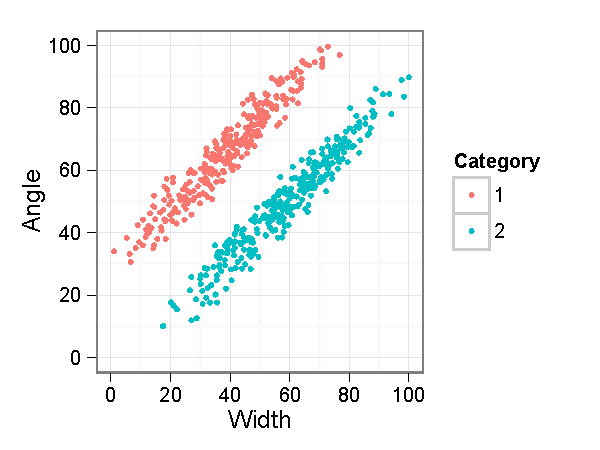
\includegraphics{f_II}
    % TODO -- replace with the good plot; find the good plot again.
    \centering
    \caption{The two sinusoidal grating distributions for the information integration (II) category distributions.   As II categories span the diagonal of the gratings parameter space (line width and angle successful learning requires consideration of both dimensions preventing participants from solving the categorization problem with simple rule-based strategies.}.
	\label{fig:II}
\end{figure}

\begin{figure}[tp]
	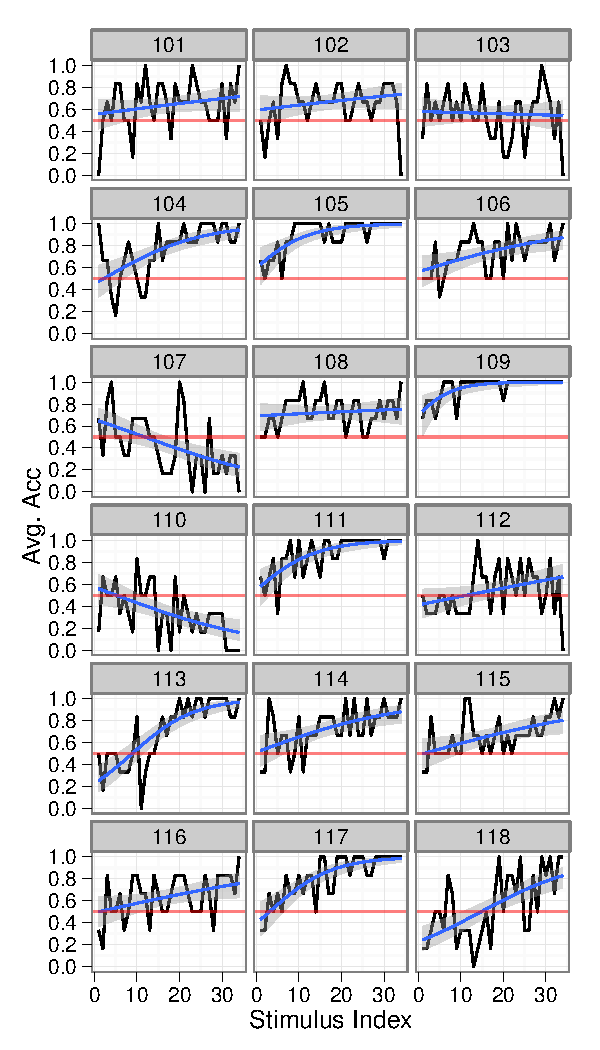
\includegraphics{f_all_sS_acc}
    \centering
	\caption{Average accuracy for each participant (black), averaged for all 6 stimuli by trial (i.e., Stimulus Index), blue line and the grey area represent a binomial regression fit of the data and bootstrapped 95\% confidence intervals, respectively.}
	\label{fig:sacc}
\end{figure}

\begin{figure}[tp]
	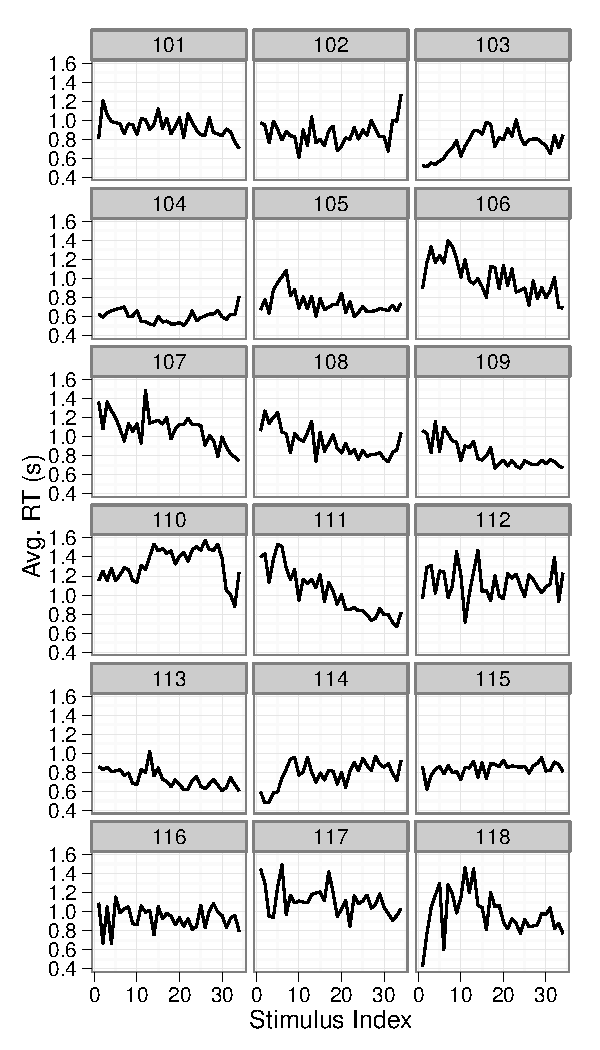
\includegraphics{f_all_sS_rt}
    \centering
	\caption{Mean reaction time for each participant, averaged for all 6 stimuli by trial (i.e., Stimulus Index).}
	\label{fig:srt}
\end{figure}

\subsubsection{Well behaved results}
\label{subsub:wellbehaved}
On an individual basis the lower confidence interval around the binomial fit of the accuracy data rose to above the chance level (0.5) by the last trial, except for participant 103, who did not learn (Figure~\ref{fig:sacc}).  Many participants (11 of 16) greatly exceeded this minimum criterion, showing above chance learning by trial 10, and nearly all (14 of 16) exceeded chance by trial 20  (Figure~\ref{fig:sacc}).  These individually good performances are reflected in the participants' aggregate performance, which was well above chance by trial 5 (Figure~\ref{fig:meanacc}).  This aggregate learning rate is consistent with past work in the lab using verbal or monetary feedback, indicating that the rewarding categories in present study are behaviorally similar to classical rewards.  The consistency between classical rewards and this task were also reflected in the reaction time measures, which showed a 200 ms decrease over time, bottoming out near 850 (for individual averages see Figure~\ref{fig:srt} and for overall performance see Figure~\ref{fig:meanrt}).  Responses in similar, classically rewarding tasks end with reaction times near 700-800 milliseconds and show similar rates of decline.  The 50-100 ms possible difference in reaction times may be due to the increased difficultly of classifying the rewards compared to simply reading the value of the outcome (e.g., ``Gain \$1'').

\begin{figure}[tp]
	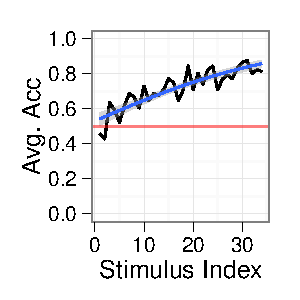
\includegraphics{f_all_mean_acc}
    \centering
	\caption{Mean accuracy (black), averaged over all participants and stimuli, plotted by trial.  The blue line and grey area represent a binomial regression fit of the data and bootstrapped 95\% confidence intervals, respectively.}
	\label{fig:meanacc}
\end{figure}

\begin{figure}[tp]
	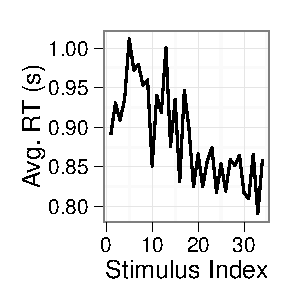
\includegraphics{f_all_mean_rt}
    \centering
	\caption{Mean reaction time (black), averaged over all participants and stimuli, plotted by trial.  The blue line and grey area represent a binomial regression fit of the data and bootstrapped 95\% confidence intervals, respectively.}
	\label{fig:meanrt}
\end{figure}

\subsection{3 Models and 2 Codes}
\label{sub:threemodels}
\subsubsection{Our three models}
\label{subsub:catquant}
Three Rescorla-Wagner models were constructed, each using a distinct reward representation.  The first model treated rewards identically to a classical reward (e.g., a 0 for a loss or 1 for a gain).  The second and third devalued each reward based on how similar it was to the category mean.  This similarity metric is (necessarily) simplistic.  As I reviewed on p\pageref{subsub:curves}, there are many proposed models for how the categories are represented.  Likewise, our understanding of the computational implementation of the category learning systems is only just underway \cite{Ashby:2005p9152,Ashby:2006p9153}.  As such there is no obvious way to interlace my hypothesis of rewarding categories with the category learning systems or with the many models of categorization they rely on.  Avoiding such ambiguity, I took a simpler route driven by Shepard's basic finding \cite{Shepard:1987p9102}.  Whatever the representation and/or category learning system that (may) implement rewarding categories, Shepard's work insists they show an exponential or Gaussian decline with similarity.  For simple stimuli like a light or tone, similarity is measured from the initial training prototype \cite{Guttman:1956p8355}.  However as my task does not have a singular prototype the mean of the parameters for all training trials (i.e., part 1) was used in its place.  This simple substitution makes my categories identical to the simplest of the prototype category representations \cite{Rosch:1973p9108,Ashby:1995p9109}, making this a parsimonious yet literature driven first attempt to quantify similarity of rewards.  Therefore, for model two similarity decreased exponentially measured from the training mean.  While for model three it decreased along a normal Gaussian (for complete mathematical detail see p\pageref{subsub:codesandfits}).  

\subsubsection{Codes and fits}
\label{subsub:codesandfits}
For each participant and model, the two free parameters ($\alpha$, which controls each model's rate of learning and $\beta$, which controls the steepness of the action selection criterion) were fit using an exhaustive\footnote{With a 0.05 precision, ranging from 0-1 for $\alpha$ and 0-5 for $\beta$} maximum log-likelihood search.  Additionally each model was run using two separate reward coding schemes.  In the first scheme Gains were valued as 1 and losses as 0.  The second, which was based on the bivalent monetary value of the rewards, uses 1 and -1 for gains and losses respectively.  The first scheme is universally used in human and animal modeling studies as well as in machine learning, and was \citeA{Sutton:1998p9247} recommended scheme.  However recent recordings of dopaminergic neurons in monkey suggest that the true reward codes are complex, even perhaps redundant \cite{Kim:2006p1063,Matsumoto:2009p7219}.  Among other schemes, they reported firing consistent with a bivalent reward code.  Using the second scheme is merely a first, albeit simple, step in incorporating the potential complexity of dopaminergic firing as observable by the fMRI BOLD signal and in human subjects.

\subsubsection{The incantations}
\label{subsub:incantations}
To restate more formally, the Rescorla-Wagner model's value updates are defined by,
\begin{equation} \label{eq:V} V(s,a,t) \leftarrow V(s,a,t) + \alpha\delta \end{equation} 
\begin{equation} \label{eq:rpe} \delta = r_{classic}(t) - V(s,a,t) \end{equation}
where $r_{classic}(t)$, i.e., the numerical representation of the rewards, can be coded as either
\begin{equation}
	\label{eq:r1}
	r_{classic}(t) = \{1,0\}
\end{equation}
or 
\begin{equation}
	\label{eq:r2}
	r_{classic}(t) = \{1,-1\}
\end{equation}
but where $r_{classic}(t)$ may also be replaced with
\begin{equation}
	\label{eq:re}
    r_{exp}(t) = r_{classic}(t)S_{exp}
\end{equation}
or
\begin{equation}
	\label{eq:rg}
    r_{gauss}(t) = r_{classic}(t)S_{gauss}
\end{equation}
where the Euclidean distance
\begin{equation}
	\label{eq:D}\\
    D = \sqrt{(\bar{\theta} - \theta)^2 + (\bar{W}-w)^2}
\end{equation}
is transformed to a Shepard-like similarity metric \cite{Shepard:1987p9102}.
\begin{equation}
	\label{eq:Sexp}\\
    S_{exp} = e^{-D}
\end{equation}
\begin{equation}
	\label{eq:Sgauss}\\
    S_{gauss} = e^{-D^2}
\end{equation}
Consistent with past work, all values are initialized at 0 \cite{Beierholm:2011p8141,BischoffGrethe:2009p4570,Gershman:2009p7207}
\begin{equation} \label{eq:V0} V_{initial}(s,t) = 0. \end{equation}
and values are transformed to response selection probabilities via the softmax distribution \cite{Sutton:1998p9247,ODoherty:2003p6329}.
\begin{equation}
	\label{eq:softmax}
	p(s_1) = {e^{\beta V(s_1,a_1,t)}\over{e^{\beta V(s_1,a_1,t)} + e^{\beta V(s_2,a_2,t)}}};\ s_1 = (s_{i},q), \ s_2 = (s_{i}, w).
\end{equation}

\subsubsection{Fits and plots}
\label{subsub:fits}
On average none of the three models fit the accuracy data better than the rest (Figure~\ref{fig:logL}).  For brevity's sake each model will be referred to as ``none'', ``exp'' and ``gauss'', corresponding to Eq~\ref{eq:rpe}, Eq.\ref{eq:re}, and Eq.~\ref{eq:rg} respectively.  Nor did the coding scheme impact the fits (``acc'' and ``gl'', matching respectively Eq.~\ref{eq:r1} and Eq.~\ref{eq:r2}; Figure~\ref{fig:logL})).  For ``acc'' the step size parameter (``alpha'' in Figure~\ref{fig:alpha} matching $\alpha$ in Eq.~\ref{eq:V}) increased in ``exp'' compared to the other models.  This increase was expected as the exponential similarity metric can sharply decrease the magnitude of each value update, requiring an increase in $\alpha$ to compensate.  A similar trend was observed for the temperature parameter (``beta'' in Figure~\ref{fig:beta}, matching $\beta$ in Eq.~\ref{eq:softmax}). The more equiprobable each action is the larger the temperature parameter.  As such the increase for ``exp'' means participant's choices are more likely to change from trial to trial, which is again consistent with a decrease in update magnitudes.

Importantly the intra-subject variability in $\alpha$ and $\beta$ was low, as demonstrated by the small standard error of both parameters (Figure~\ref{fig:alpha} and~\ref{fig:beta}).  Consistent parameter estimates between subjects support my use of subject-level parameters in the fMRI analyses, which in other hands have been reported to be too noisy to be reliable \cite{Daw:2011p7995,Seymour:2007p7585,ODoherty:2003p6329}.  I believe, using subject-level parameters is a step crucial in assessing and maximizing model quality. The goal of any model of human behavior is to make good predictions for individual cases not just for aggregates of tens or hundreds of participants \cite{Daw:2007p9346}.  However aggregates prediction is the norm in reinforcement learning models of human behavior (for examples see, \citeA{Daw:2011p7995,Seymour:2007p7585,ODoherty:2003p6329}).

\begin{figure}[tp]
	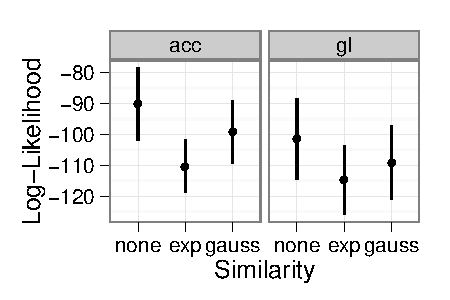
\includegraphics{f_logL}
    \centering
	\caption{Average negative log-likelihoods for each of the models and coding schemes.  Error bars represent standard errors.}
	\label{fig:logL}
\end{figure}

\begin{figure}[tp]
	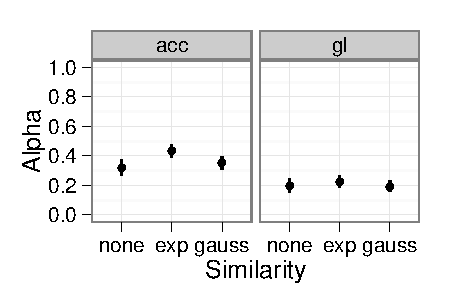
\includegraphics{f_alpha}
    \centering    	
    \caption{Average alpha values for each of the models and coding schemes.  Error bars represent standard errors.}
	\label{fig:alpha}
\end{figure}

\begin{figure}[tp]
	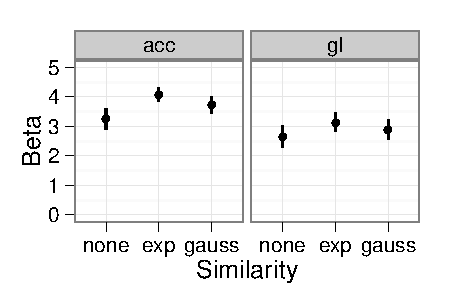
\includegraphics{f_beta}
    \centering
	\caption{Average beta values for each of the models and coding schemes.  Error bars represent standard errors.}
	\label{fig:beta}
\end{figure}

The fit reinforcement learning models for every participant and coding scheme can be found in Figure~\ref{fig:rpeacc} -~\ref{fig:valuegl}.  In the traditional formulation, where similarity does not impact reward value (e.g., see Figure~\ref{fig:rpeacc} or~\ref{fig:rpegl}) the reward prediction error decreases with learning, eventually plateauing at 0, for strong examples see subjects \emph{102}, \emph{105} and \emph{111} in the ``none'' column of Figure~\ref{fig:rpeacc}.  In contrast, both similarity models, ``exp'' and ``gauss'', never fully plateaued (again see Figure~\ref{fig:rpeacc}).  In the context of the models, this is expected.  Each grating will, in all likelihood, be non-identical to the mean. However as the parameter mean is the asymptotic expectation, reward prediction errors happen even after learning is complete.  In the big picture, this is desired model behavior.  The similarity adjusted model's are trying to capture the case where a reward's value may vary in ways that are not predictable \emph{a priori} given the massive multiplicity of possible outcomes it is unlikely to find the same one multiple times.  Small prediction error should then continue without end, as happens in these models.

When comparing ``exp'' and ``gauss'' models, you'll see the former appears to have lower magnitudes (Figure~\ref{fig:rpeacc}).  Examining density plots composed of all participants data confirms this observation (Figure~\ref{fig:denrpe}).  The density plot also reveals that ``exp'' prediction errors are diminished more rapidly than their ``gauss'' counterparts (a pattern most clearly scene in the left panel of Figure~\ref{fig:denrpe}).  

Regardless of model class, between the two reward codes there are substantial differences in reward prediction behavior.  The $\{1,-1\}$ (denoted in these plots as ``gl'') scheme leads to substantially more negative deflections that the $\{1,0\}$ scheme (``acc'') (compare Figure~\ref{fig:rpegl} and ~\ref{fig:rpeacc} as well as the \emph{left} and \emph{right} panels of~\ref{fig:denrpe}).   

Value estimates for the two similarity adjusted rewards (i.e., ``exp'' and ``gauss'') were generally less than the alternative classic model (``none'' in Figure~\ref{fig:valueacc} and~\ref{fig:valuegl}).  However, as consequence of their reduced dynamic range, the similarity adjusted model's value terms grew more rapidly, for example examine participants \emph{105} and \emph{109} in Figure~\ref{fig:valueacc}.  In these cases both the similarity value terms approached their maximum by trial 50 whereas ``none'' (the unadjusted term) took until trial 150.  That is, taking into account the uncertainty of each reward's worth lead to an increase in the learning rate.  This increase was independent of the reward coding scheme (i.e., see also Figure~\ref{fig:valueacc}-~\ref{fig:valuegl}).  

The coding scheme's impact on the value terms was two fold.  First, as losses lead to larger prediction errors using the ``gl'' scheme (-1 compared to 0), value increased faster for ``acc'' (see Figure~\ref{fig:valueacc} and~\ref{fig:valuegl} as well as~\ref{fig:denvalue}).  Second, and most strikingly, ``gl'' lead to negative value estimates of the undesirable choices (Figure~\ref{fig:valuegl} compared to~\ref{fig:valueacc}).  While, so far as I'm aware, no reinforcement learning model of human or animal have considered negative value estimates, there is empirical support.  As reviewed on p\pageref{subsub:fclt}, orbital frontal and ventral medial frontal cortices encode the absolute value of rewarding or punishing outcomes \cite{ODoherty:2001p2423,Hornak:2004p6234}.  As such, neural correlates of reinforcement learning derived negative value estimates might serve as an important link between theoretical and empirical findings on economic valuation.  It might also serve as a link between reinforcement learning and affective/motivational processing \cite{Knutson:2005p1627,Delgado:2004p6665}.

\begin{figure}[tp]
	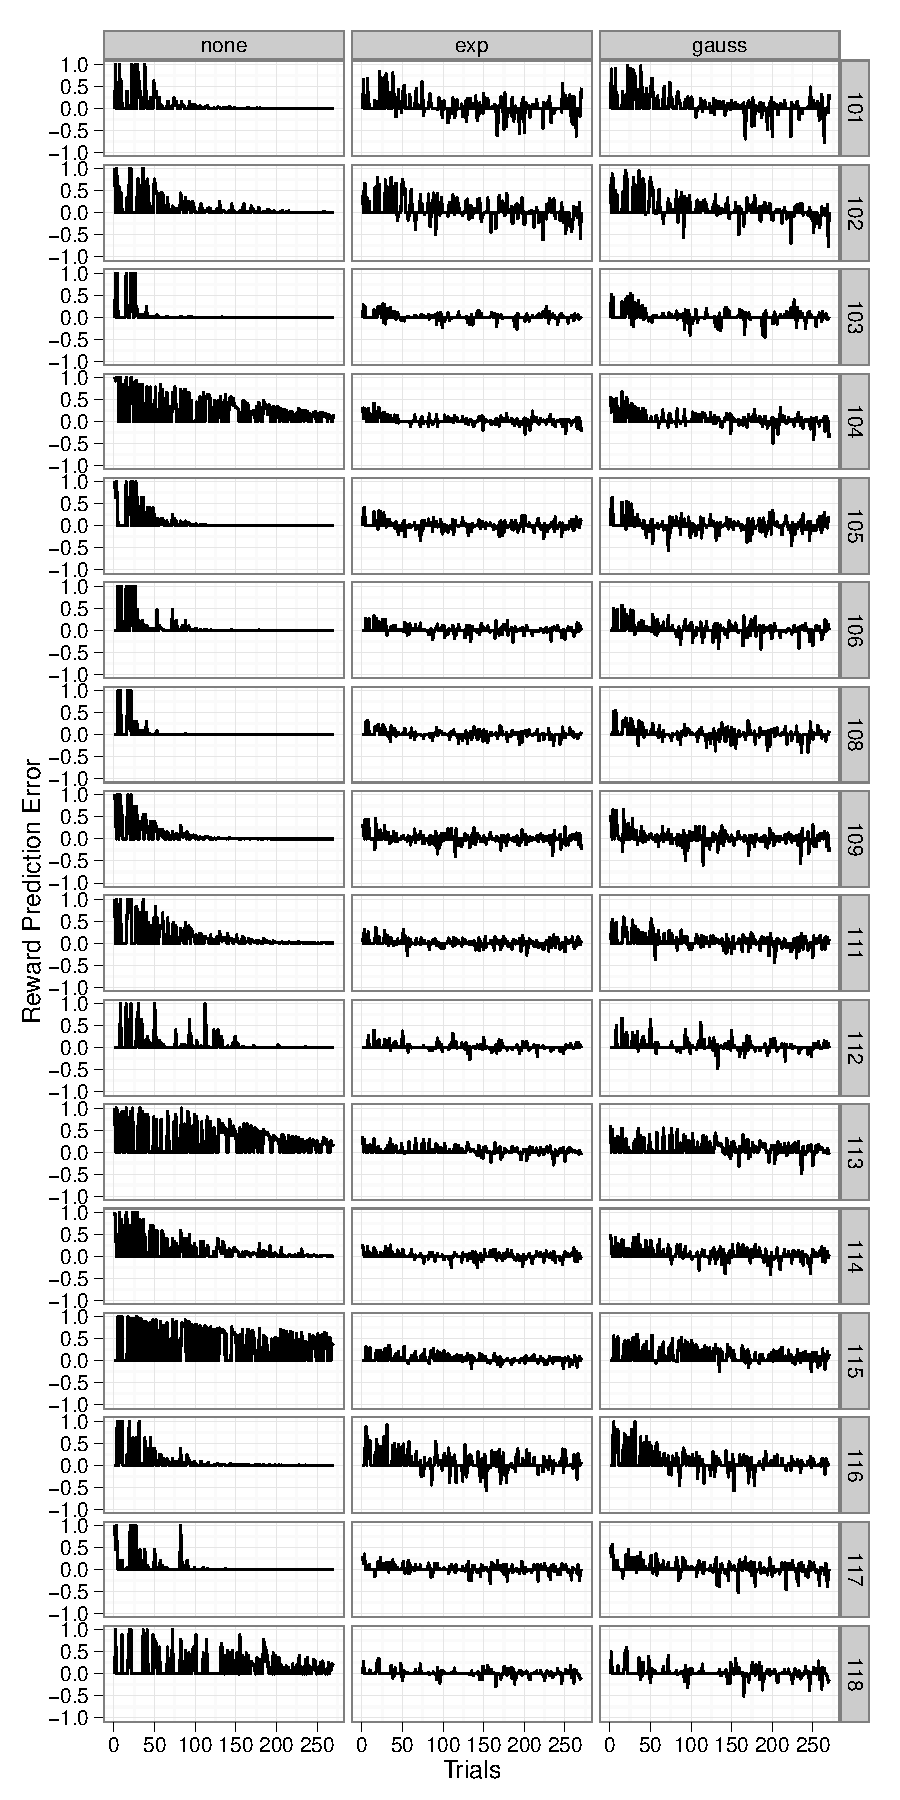
\includegraphics[width=0.6\textwidth]{f_rpe_acc}
    \centering
	\caption{Reward prediction errors for each of the three models plotted for each trial in the experiment, based on the $\{1,0\}$ coding scheme.  Each row is a single subject's data.  Each column matches one of the three models, classified by their similarity metric.}
	\label{fig:rpeacc}
\end{figure}
\begin{figure}[tp]
	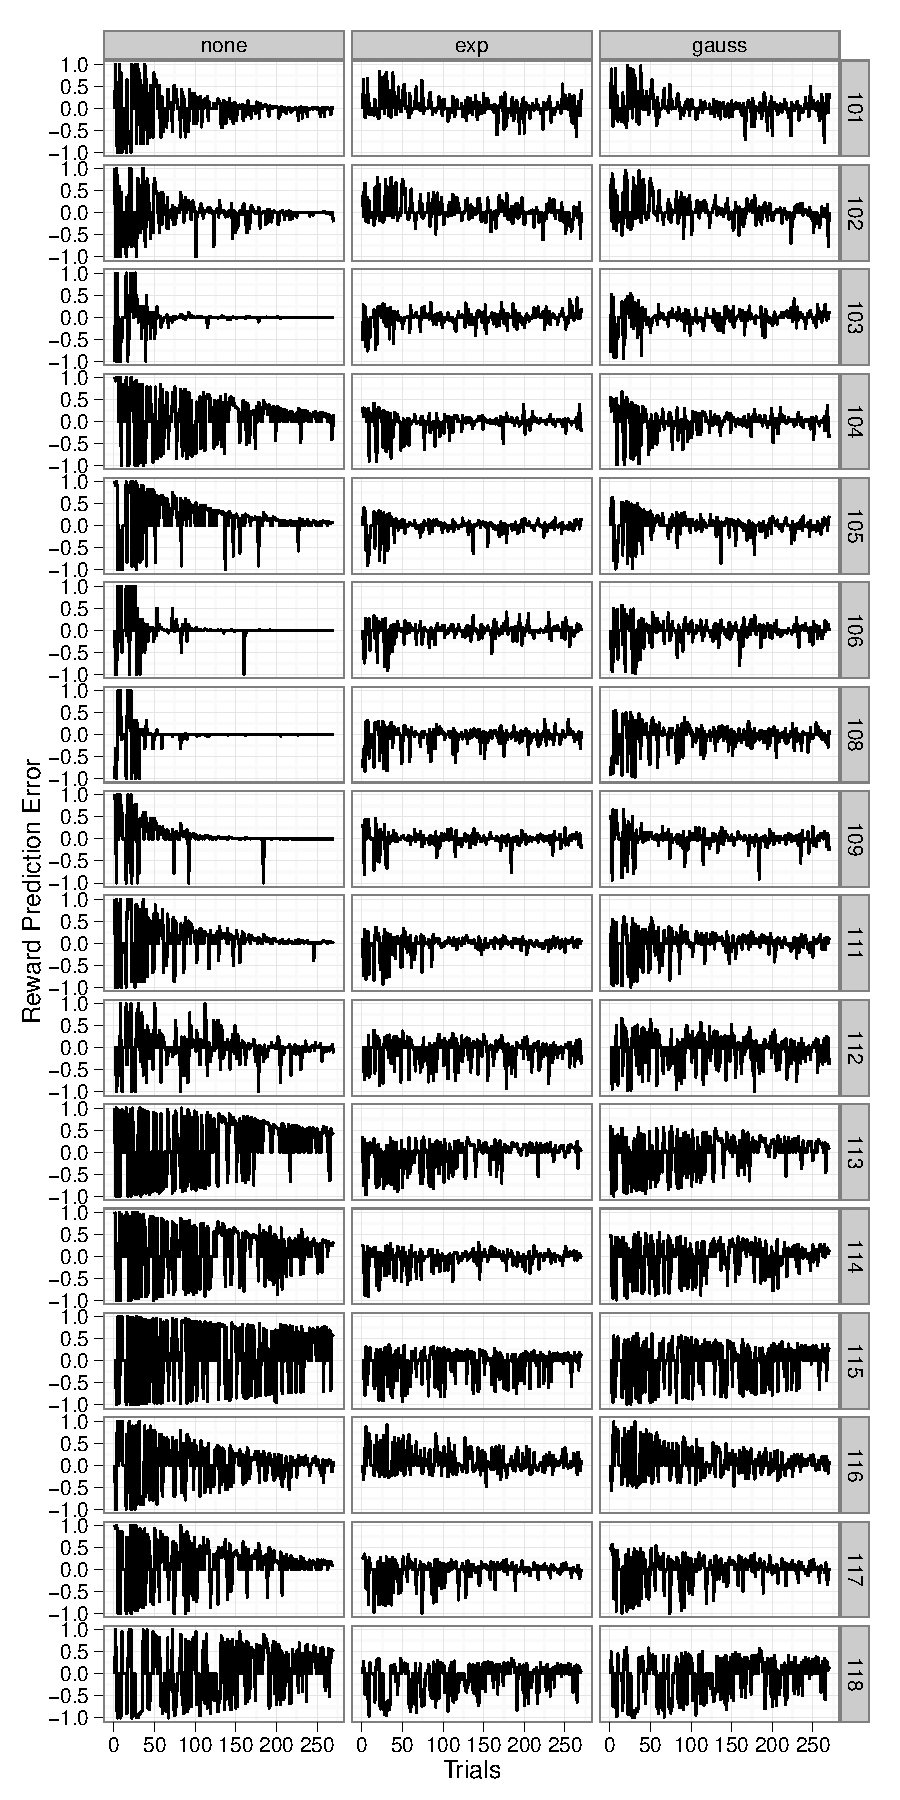
\includegraphics[width=0.6\textwidth]{f_rpe_gl}
    \centering
	\caption{Reward prediction errors for each of the three models plotted for each trial in the experiment, based on the $\{1,-1\}$ coding scheme.   Each row is a single subject's data.  Each column matches one of the three models, classified by their similarity metric.}
	\label{fig:rpegl}
\end{figure}

\begin{figure}[tp]
	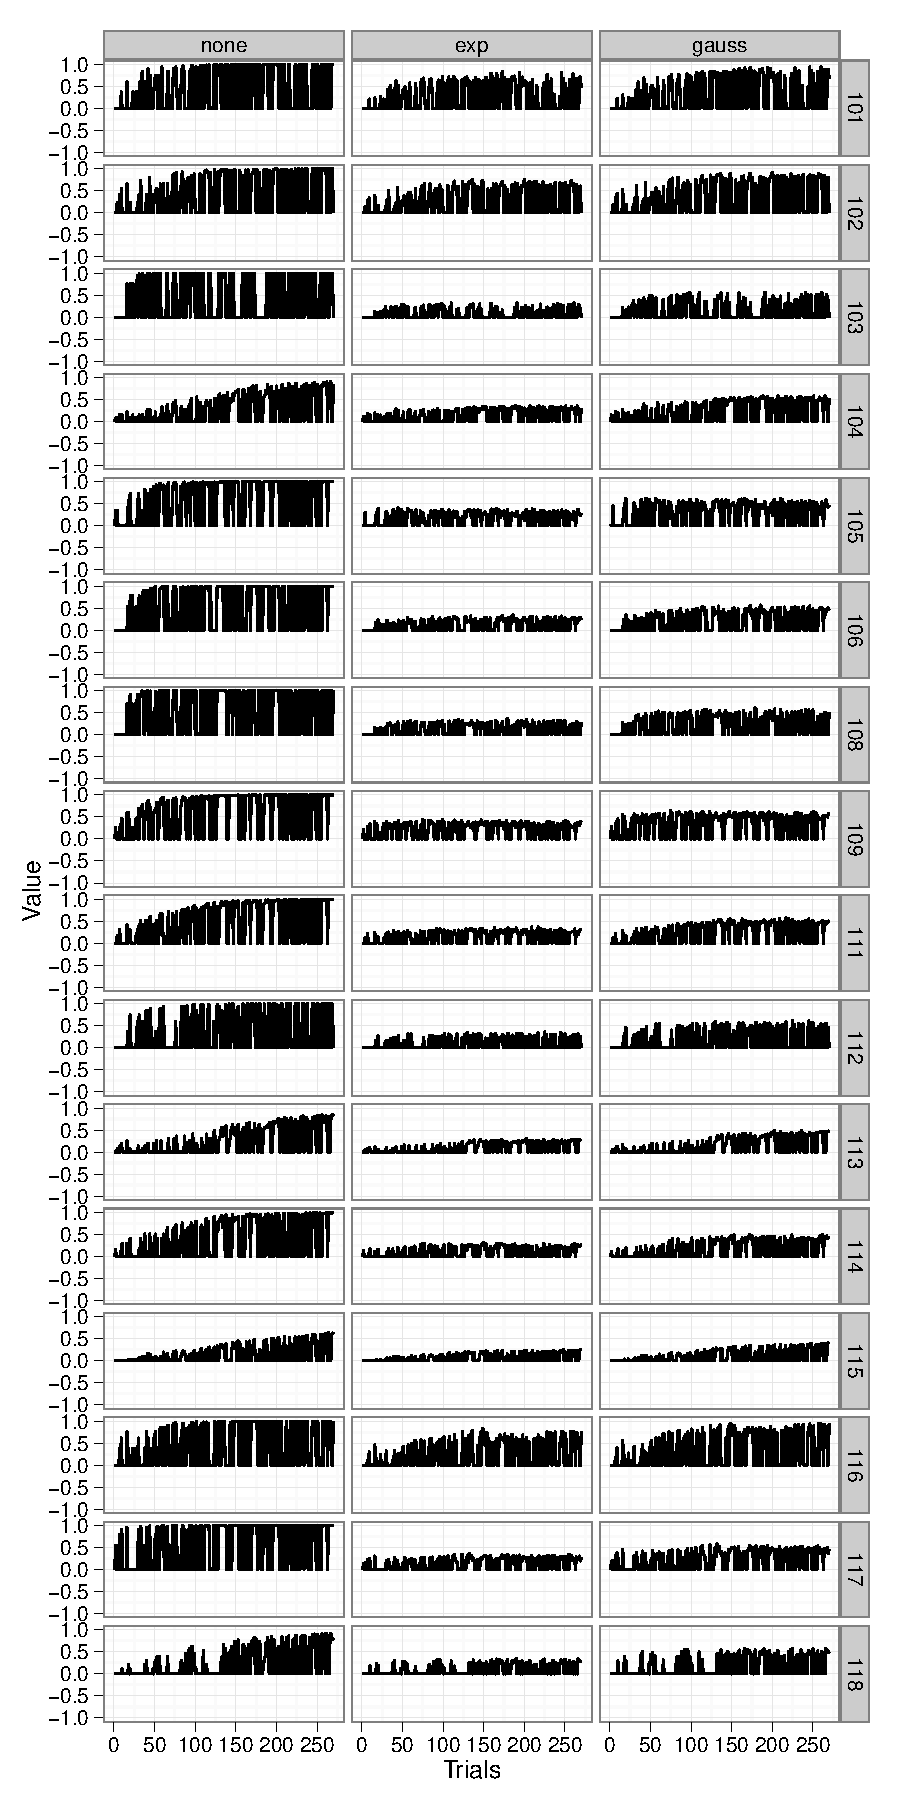
\includegraphics[width=0.6\textwidth]{f_value_acc}
    \centering    
	\caption{Value estimates for each of the three models plotted for each trial in the experiment, based on the $\{1,0\}$ coding scheme.  Each row is a single subject's data.  Each column matches one of the three models, classified by their similarity metric.}
	\label{fig:valueacc}
\end{figure}
\begin{figure}[tp]
	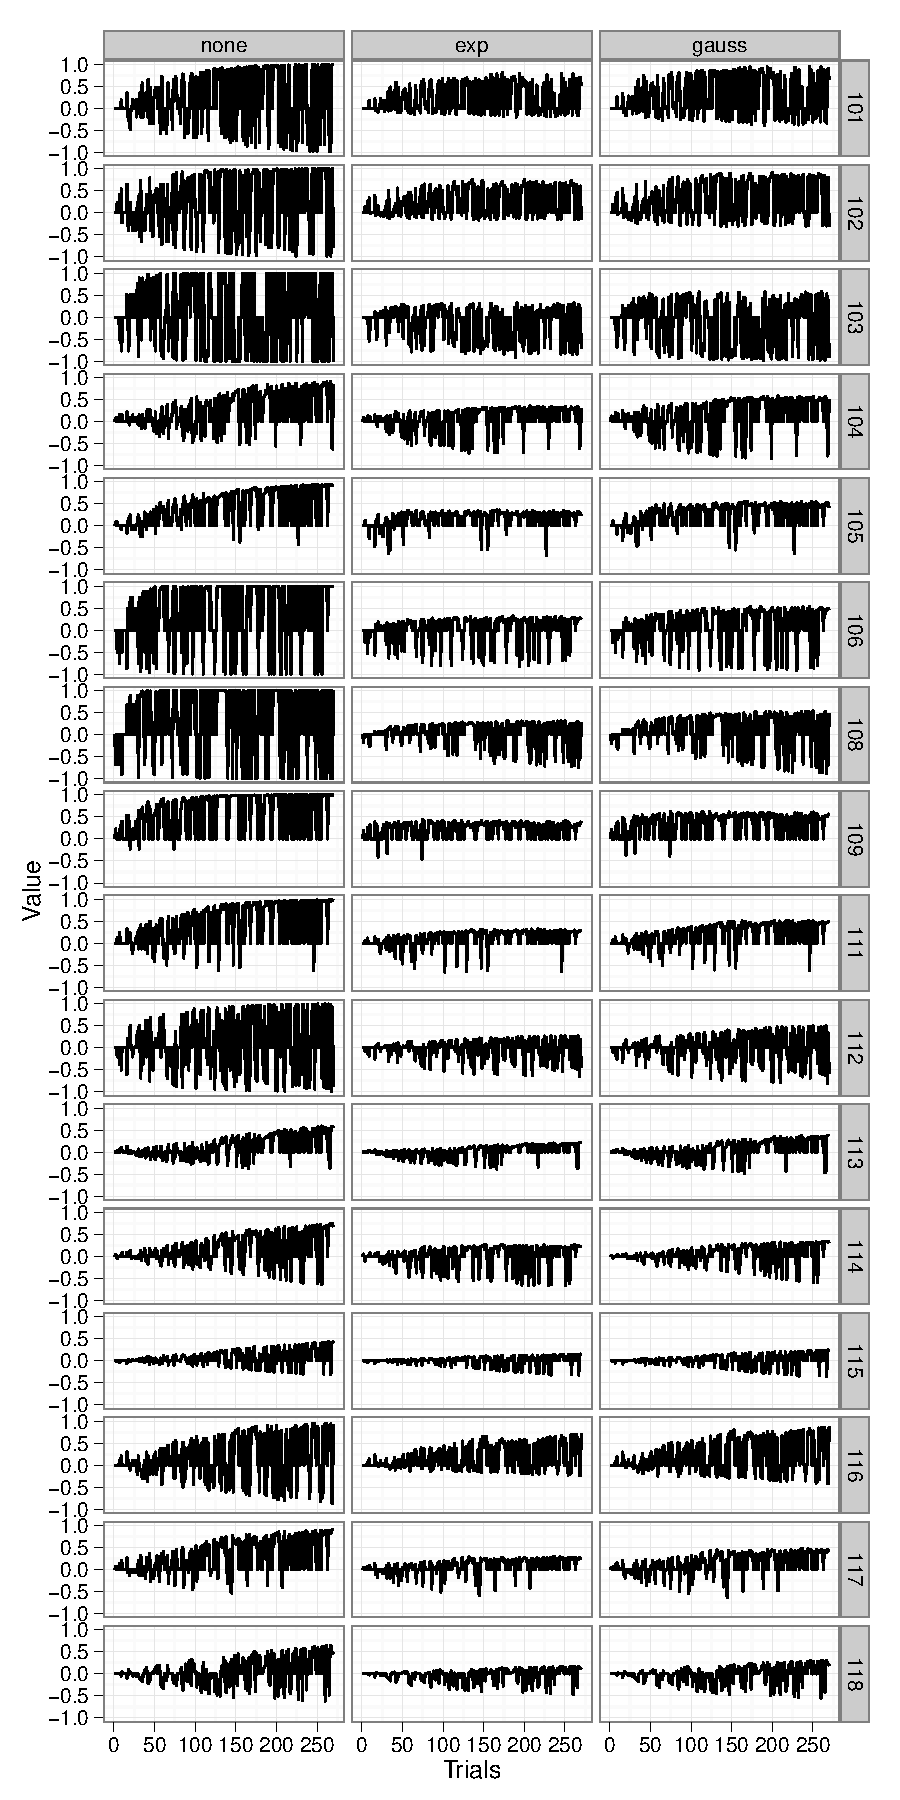
\includegraphics[width=0.6\textwidth]{f_value_gl}
    \centering
	\caption{Value estimates for each of the three models plotted for each trial in the experiment, based on the $\{1,-1\}$ coding scheme.   Each row is a single subject's data.  Each column matches one of the three models, classified by their similarity metric.}
	\label{fig:valuegl}
\end{figure}
\begin{figure}[tp]
	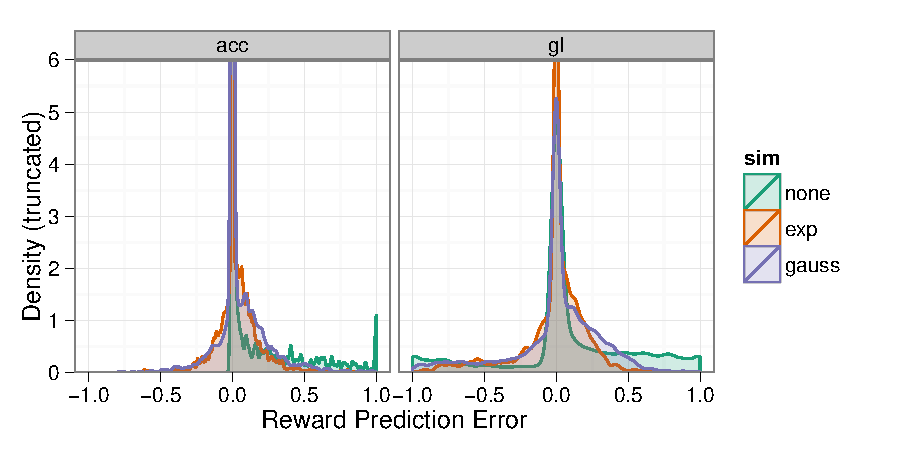
\includegraphics{f_density_rpe}
    \centering
    \caption{Density of reward prediction errors for all subjects.  The y axis is truncated at 6 to allow clear visualization of non-zero values.}
	\label{fig:denrpe}
\end{figure}

\begin{figure}[tp]
	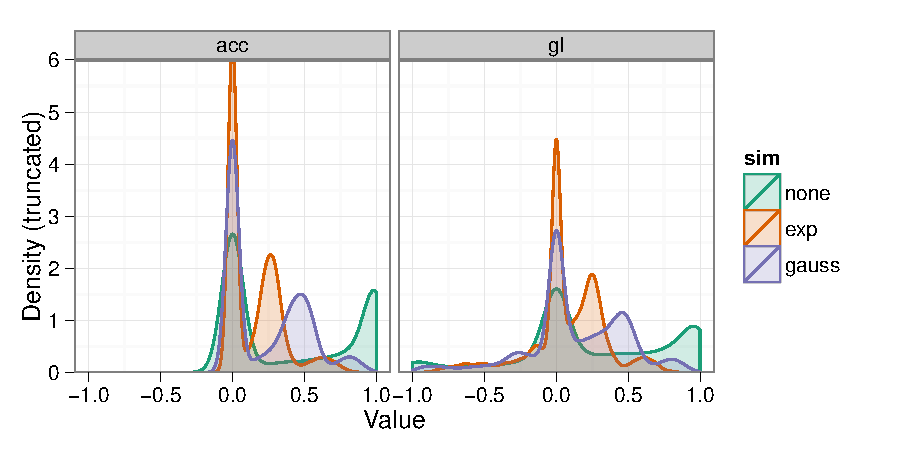
\includegraphics{f_density_value}
    \centering
    \caption{Density of value estimates for all subjects.  The y axis is truncated at 6 to allow clear visualization of non-zero values.}
	\label{fig:denvalue}
\end{figure}

\clearpage
\newpage
\section{Chapter 3 -- fMRI analyses} % (fold)
\label{sec:task_and_models}
\subsection{An Acquisition}
\label{sub:acquired}
\subsubsection{Data details}
\label{subsub:datadetails}
fMRI data was acquired at the Intermountain Neuroimaging Consortium (INC) facility located at the University of Colorado at Boulder on a Siemens Allegra 3T (whole body) scanner.  All 18 right-handed participants were pre-screened for the typical fMRI exclusion factors (e.g., metal implants, mental disorders, etc).  High resolution anatomical data was acquired as a T1-weighted structural image, MPRAGE sequence, at 1x1x1 mm, (256 x 156 x 192) with a TR of 2530 ms, and TE of 1.64 ms, with a flip angle of 7$^\circ$.  All functional (i.e., BOLD) data was acquired with T2-weighted echo-planar imaging (EPI), at 2.29 x 2.29 x 4.00 mm (96 x 96 x 26), with a TR of 1500 ms, a TE a 25 ms, a flip angle of 75$^\circ$ and a FOV of 220 mm.

Four sets of functional data were acquired.  The first was of the ``refresher'' for part 1 of the behavioral training (p\pageref{subsub:whatwhen}), spanning 241 volumes.  The second and third spanned part 2 of the stimulus-responses learning task, divided into 2 (nearly) even sets lasting 390 and 394 volumes respectively (again see p\pageref{subsub:whatwhen}).  The fourth scan featured repeated presentation of gratings from both reward categories, in a random order.  The intent of this scan was to isolate rewarding activity outside the primary task. This localizer was not in the end useful (discussed on p\pageref{subsub:chunks}).

\subsubsection{Preprocessed (model) food}
\label{subsub:preprocessed}
Following DICOM to nifiti-1 conversion using dicom2nii (\url{http://www.mccauslandcenter.sc.edu/mricro/mricron/dcm2nii.html}), each dataset was subjected to the following preprocessing pipeline carried out in SPM8's batch mode (\url{http://www.fil.ion.ucl.ac.uk/spm/software/spm8/}).  For complete code see, \url{https://github.com/andsoandso/fmri/tree/master/catreward/spm\_m}.  Anatomical data was first segmented into white and grey matter regions \cite{Collignon:1995p9347}.  Based on these segments the parameters necessary for normalization into a standard reference space (T1 MNI-352, at 1 mm, MNI space or short) were calculated. Normalization had two steps.  The first was a Bayesian 12-parameter affine transformation \cite{Ashburner:1997p9348}.  The second was a set of nonlinear deformations, using a 1127 parameter discrete cosine transform \cite{Ashburner:1999p9350}.  Anatomical data was then resampled from 1.27 to 1.00 $mm^3$ using fourth degree $\beta$-splines, and finally, using the parameters above, normalized into MNI space.

To correct for the slight head movements that often occurring during scanning, movement regressors for all volumes of the functional data were first calculated \cite{Ashburner:1999p9350}.  No participant moved more than 1.5 mm, so all data was retained.  Functional data was then slice-time corrected, using slice 13 (the middle slice from the descending acquisition) as the reference, followed by coregisteration with the pre-processed (native-space) anatomical data, and resampling into 3 mm$^3$ voxels, again using fourth degree $\beta$-splines \cite{Collignon:1995p9347}.  Functional data was then normalized into MNI space using the anatomically-derived parameters above.  Finally, the functional data was spatially smoothed using a 6 mm FWHM Gaussian, though a copy of the unsmoothed data was retained for the ROI analyses (described on p\pageref{sub:regoins}).  Just prior to regression analysis, each voxel's time course was also low-pass filtered using finite impulse response model, with a cutoff at 0.008 Hz \cite{Kruggel:1999p9351}.  For all whole-brain analyses, the movement regressors were entered into the regression models as covariates, accounting for any head movement.  Given the large spatial averages employed in the ROI analyses these weren't motion corrected \cite{Poldrack:2007p8572}.

\subsubsection{The best of all possible signals}
\label{subsub:bestsignal}
In fMRI, and in general time-series analysis, there is an intrinsic trade-off between detecting a signal in the presence of noise and estimating the shape of that signal \cite{Dale:1999p7901,Birn:2002p1777,Liu:2004p2141}.   One way to optimize over both these conflicting objectives is to manipulate the trial order in a rapid event-related design \cite{Miezin:2000p7924}.  One state-of-the-art method for optimizing the trial ordering process is a genetic algorithm which uses two (weighted) loss functions, one for signal detection and one for time-course estimation \cite{Wager:2003p2980}. \citeA{Kao:2009p7899}, improved on Wager's (2003) initial design by adding in a loss function for psychological considerations, greatly improving execution speed and documentation.  As a result, Kao et al's (2009) method/code was used to optimize trial orders for part 1 and 2 of the behavioral task (p\pageref{subsub:whatwhen}), along with the reward category localizer scan (p\pageref{subsub:datadetails}).

\subsection{Mobs of Blobs}
\label{sub:blob}
All statistical parametric maps (below) were derived from a Random Effects analysis (RFX, or ``second-level'' in SPM8 jargon), multiple comparison corrected assuming Gaussian Random Fields using the Family Wise Error Rate (FWE) at the $p < 0.05$ level, with a minimum cluster size of 4 voxels \cite{Worsley:1996p9367}. 

Whole brain activity for the stimulus-response learning portion of the behavioral experiment (i.e., part 2, p\pageref{subsub:whatwhen}) was examined first by comparing all trials to the baseline (rest) condition.  This data is presented in two ways. First is the statistical thresholded image.  This contrast map showed significant bilateral activity in the cerebellum, insula and anterior cingulate ($t$(15) = 6.59, $p< 0.05$; Figure~\ref{fig:gl}).  Second is an overlay of the raw $t$-values, which allows for visual confirmation the observed significant effects were robust and widespread in their respective regions, but also allowed for the analysis of overall and sub-threshold patterns of activity.  These raw data suggested near threshold levels of activity in the head of the caudate, ventromedial, dorsolateral frontal cortices as well as (weaker) activity in the occipital lobe (Figure~\ref{fig:glraw}).  And indeed in a two-way ANOVA looking at that interaction between gains and losses, significant clusters were observed in head and body of caudate, insula, posterior and anterior cingulate with the posterior activation extending into the precuneus, as well as in dorsolateral (i.e middle frontal) PFC, and in ventrolateral PFC (Figure~\ref{fig:gxl}; $F$(1, 270) = 30.76, $p < 0.05$).  When gains and losses were examined separately, but again compared to rest, both had activity in the same areas as in the combined condition (not shown).

\begin{figure}[tp]
	\fitfigure{f_map_gl_p05}
    \centering
    \caption{Statistical parametric map for all trials in the stimulus-response learning task (i.e., part 2, p\pageref{subsub:whatwhen}), compared to the rest period.  \emph{Left} is a glass brain, showing all significant clusters.  \emph{Right} is a set of axial slices highlighting strong areas of activity overlaid onto the T1 MNI-352 template.  $Z$ is the height of the axial slice in MNI space.}
	\label{fig:gl}
\end{figure}

\begin{figure}[tp]
	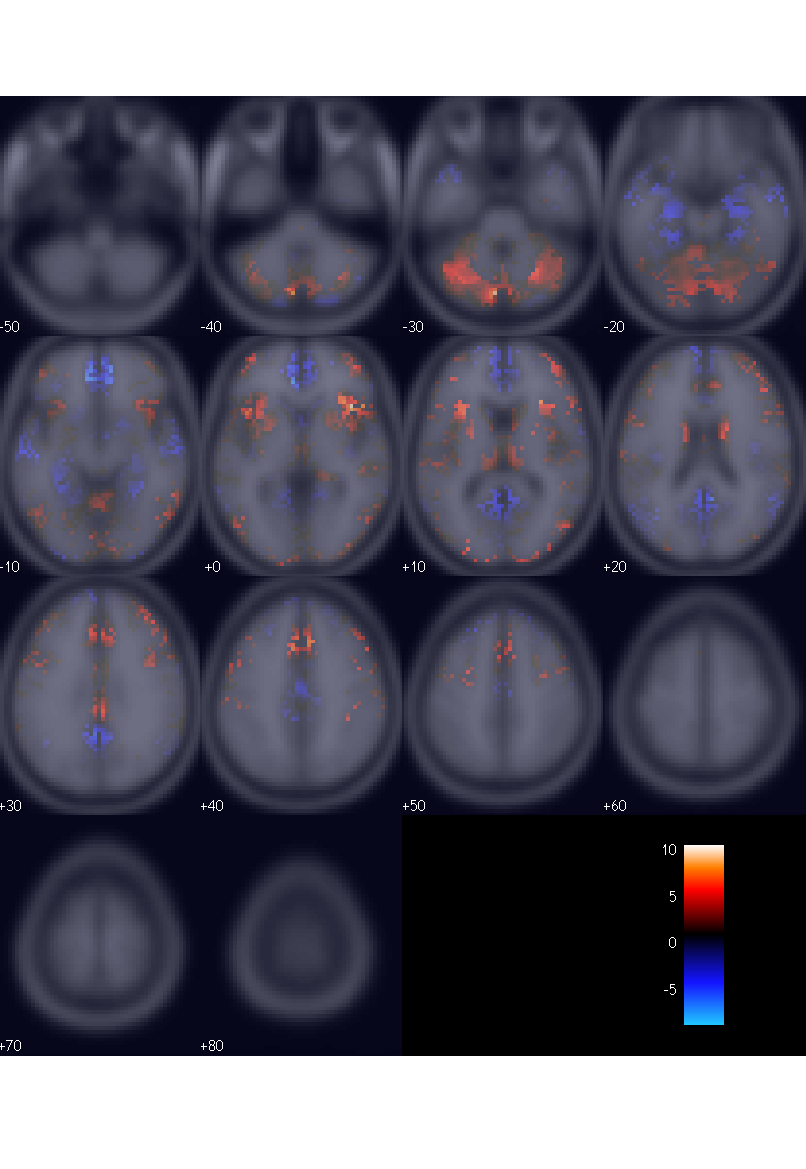
\includegraphics{f_map_gl_raw_t}
    \centering
	\caption{(The $t$-values for all trials in the stimulus-response learning task (i.e., part 2), compared to the rest period,  overlaid onto the T1 MNI-352 template.   Each number is the height of the axial slice in MNI space.}
	\label{fig:glraw}
\end{figure}

\begin{figure}[tp]
	\fitfigure{f_map_gxl_p05}
    \centering
	\caption{Statistical parametric map for all trials in the stimulus-response learning task (i.e., part 2) examining the interaction between gains and losses.  \emph{Left} is a glass brain, showing all significant clusters.  \emph{Right} is a set of axial slices highlighting strong areas of activity overlaid onto the T1 MNI-352 template.  $Z$ is the height of the axial slice in MNI space.}
	\label{fig:gxl}
\end{figure}

\subsection{Regions and Models}
\label{sub:regoins}
\subsubsection{The right chunks}
\label{subsub:chunks}
Following whole-brain analysis, regions of interest were selected using two separate yet related methods.  The first employed only regions from the Harvard-Oxford probabilistic anatomical atlas, using the 50\% cutoff \cite{Desikan:2006p9370}.  The second combined anatomical regions with functional clusters isolated using both the data collected during the second half of part 1 (i.e., the ``refresher'') and from the reward category localizer (p\pageref{subsub:datadetails}).  Comparisons between them showed the anatomically-limited functional clusters and the entire anatomical regions displayed very similar results.  So to limit the complexity of later analyses, and to increase power, functional clusters were discarded in favor of the larger anatomical regions.  Most anatomical regions of interest were selected \emph{a priori} based on previous studies of reinforcement and category learning (see the \emph{Introduction} for a review).  Left and right subcortical regions of interest were the dorsal caudate, ventral striatum/nucleus accumbens, and putamen.   Bilateral cortical areas were the middle frontal cortex (i.e., dorsolateral PFC), frontal medial cortex (which contains ventrolateral PFC), and orbital frontal cortex.  Based on the whole-brain maps (p\pageref{sub:blob}), regions for the insula, anterior and posterior cingulate (ACC and PCC for short) were included as well. While I've no strong \emph{a priori} hypothesis for the role of these regions may play or may not play, activity in each of these \emph{post hoc} regions is common to human category learning experiments \cite{LopezPaniagua:2011p8296,Seger:2010p7188,Cincotta:2007p6672,Seger:2006p5447,Seger:2005pd}.


% -- PROOFED ABOVE
\subsubsection{A way to(o) many}
\label{subsub:tomany}
There are 6 models under evaluation: the three kinds of similarity adjustment (``none'', ``exp'', and ``gauss'') multiplied by the two possible reward codes (``acc'' and ``gl''), with the two terms of interest (i.e., value and the reward prediction error), that is 12 comparisons.  The were also a number of \emph{a priori} confounds to our signals of interest including the similarity metrics, the reward codes, and the grating parameters, bringing the total to 23.  As the models are not nested\footnote{
    Often defined by whether or not two models can be made identical by adding or subtracting parameters \cite{Forster:2000p9623}} and therefore not amenable to $F$-tests -- the common statistical way to compare model fits -- an alternative approach was called for.  Further complicating the issue was the fact that each of the models is covariate, if not collinear, with the others.  To top it off, none of the three similarity-adjustments are statistically independent; reinforcement learning can be viewed as a regression of the reward code onto behavioral choices.  All these factors combined would make statistical testing difficult, to say the least.  But fortunately finding \emph{the} best model is not the goal.  

The latest recordings of phasic (i.e., reward prediction) activity in the VTA/SNc suggests a complicated reward and prediction error coding scheme (see p\pageref{subsub:expectations}), wherein several separate sets of calculations may be carried out independently \cite{Kim:2006p1063, Matsumoto:2009p7219, Smith:2011p8133}.  The observed BOLD signal is then an aggregate of these many activities. It is possible, even likely, then that more than one of the models is correct making null hypothesis tests an incorrect choice.  Model selection is the right choice.

Model selection is the process of finding a \emph{family} of models that best predict a given dataset \cite{Rao:2001p9457}.  Most techniques try to wisely balance parsimony with increasing fit (i.e., solving the bias versus variance dilemma \cite{Geman:1p9469}).  Unfortunately most model selection techniques require assumptions my models cannot meet (e.g., statistical independence).  The few that can tend to be complex recent statistical inventions.  Rather than navigate those troubled and unproven waters, I took a simpler approach. Each model was independently examined and ranked, in an approach loosely similar to model averaging \cite{Forster:2000p9623}.

An AIC score (Akaike Information Criterion \cite{Akaike:1974p9530}) was assigned to each of the models/codes for every participant and region of interest.  The absolute AIC score across participants is not however meaningful.  Only the relative values are of interest \cite{Wagenmakers:2004p9472}.  As a result, individual's scores were normalized and ranked by subtracting the best (lowest) score from each \cite{Anderson:2000p9475}. The normalized set was then transformed to Akaike Weights, a way to easily compare the conditional probabilities of each model being true \cite{Wagenmakers:2004p9472}.  The Akaike Weights were then averaged across participants for each model and region of interest.

\subsubsection{Information on information}
\label{subsub:way}
AIC is a measure of loss; how much information is lost by substituting the model for the true distribution, i.e., the data.  The lower the AIC score, the better the model.  Unlike null hypothesis tests and Bayesian measures, AIC-based methods do not seek to find \emph{a} truth, but instead serve to rank models.  AIC offers then only relative insight, and is unable to make any claims about absolute significance.  Significance is a separate question, one I'll return to later.  Besides this limitation, AIC has some substantial advantages. Five are reviewed below.

One, unlike maximum-likelihood, AIC is designed to be a parsimonious score.  It penalizes for additional parameters.  It may therefore choose a worse model (as measured by likelihood or mean squared error) over a better but more complex one. This is the essence of Occam's razor\footnote{Famously and pithily expressed as, ``Entities are not to be multiplied beyond necessity''.}. 

Two, it fits with the process of science.  When designing an experiment it is rare that there are only two possible outcomes, instead typically there are several competing hypothesis, some of which may not be mutually exclusive.  AIC's focus on relative differences and evidential weights meshes perfectly with the reality of multiple working hypotheses \cite{Burnham:2004p9621}.

Three, truth can remain elusive.  A common alternative to AIC is BIC, the Bayesian Information Criterion.  Like AIC, BIC is derived from the log-likelihood of a model, however its derivation requires a rather strict (and often unrealistic) assumption -- that the true model is among the candidates \cite{Forster:2000p9623}.  And while it may be philosophically debatable whether any mathematical model can \emph{completely} describe reality, in this study I know my models are incomplete.  As, one, the human reinforcement learning literature contains several recent theoretically unaccounted for findings and, two, there are theoretical developments I do not include here to keep the models tractable (see the \emph{Introduction} for a review).  

Four, AIC values are easily interpretable once they're transformed to Akaike Likelihoods or Weights\footnote{
    Likelihood for model $k$ among $K$ working hypotheses/models is given by $L_k = e^{-0.5({AIC}_k - {min}_{K}{(AIC)})}$, which is then normalized, becoming an Akaike Weight by $w_k = L_k / \sum\limits_{k=1}^K L_k$ \cite{Burnham:2004p9621}.}.  The likelihood is, as you would expect, simply the likelihood the model is correct (based on the information loss associated with it), while the Akaike Weights are normalized likelihoods.  As the Weights sum to one, the conditional likelihood of one model compared to another is just the ratio of their weights \cite{Burnham:2004p9621}.  For example, the conditional likelihood of model A over model B is just $w_A/w_B$.  That is, the likelihoods and Akaike Weights are intrinsically measures of effect size \cite{Anderson:2000p9475,Forster:2000p9623}.  Despite the fact that it is often used to express the likelihood of correctly rejecting the null hypothesis, the $p$ value is not a measure of effect, as $p$ is contingent not just on effect size but on sample number.  
    
    Five, AIC has a history with models of categorization. \citeA{McKinley:1996p9532,Maddox:2001p9533}, among several others, used AIC to compare behavioral results to several alternative models of categorization.  

\subsubsection{F-them}
\label{subsub:F}
AIC ranks offer no information about significance, in the familiar null hypothesis sense, or about the absolute fit of the model.  I addressed both of these in a series of $F$-tests run prior to AIC analysis.  These (fixed-effect, across participant) omnibus tests asked whether the total set of regression parameters for each linear model (described below) could explain the BOLD time series better than chance (i.e could the null hypothesis (of 0) be rejected).  Keeping with recommendations of \citeA{Burnham:2004p9621, Forster:2000p9623}, who argue that as AIC and significance tests are so dissimilar that direct comparison/interaction between them will be at best misleading, the models are not discarded based on significance.  All models are retained, and later AIC ranked.  The $F$-tests are a separate measure whose results are integrated during interpretation, not during model selection.

\subsubsection{Code, BOLD, and models.}
\label{sub:cmb}
A total of 23 models were compared for each of the 12 regions of interest for each of the 16 subjects, 4416 comparisons in total.  Each of the models is described below (Table 1).  In general, a time-series (e.g the reward prediction error for each trial or the similarity for that trial's outcome) was convolved with a ``canonical''  haemodynamic response function, a mixture of gamma functions that serves as a parsimonious estimate of the (instantaneous) BOLD response \cite{Friston:1998p2022}.  The convolved series was then low-pass filtered, matching the treatment of the BOLD data (p\pageref{subsub:preprocessed}).  Each convolved and filtered model was then regressed onto the BOLD response for each participant's region of interest, retaining all parameters and fit measures inside subject-level HDF5 files.  The HDF5 format offers high performance read/write operations, and widespread support across several scientific programming languages (\url{http://www.hdfgroup.org/HDF5/}).

No available fMRI analysis package returns AIC scores (or measures that could be converted to such) and none allow for the efficient (i.e programmatic) analysis of many competing computational models. So I created a region of interest focused fMRI analysis tool in Python (v2.7.1) to meet those two needs.  This module, simply named ``roi'', has since been release under the BSD license and is available for download at \url{https://github.com/andsoandso/roi}. It relies on the nibabel library to read the nifiti-1 files  (v1.2.0; \url{http://nipy.org/nibabel}), nitime for time-series analysis, (v0.4; \url{http://nipy.sourceforge.net/nitime/}) Numpy for generic numerical work (v1.6.1; \url{http://numpy.scipy.org/}), with the GLS function from the scikits.statsmodels module handling the regressions (v0.40; \url{http://statsmodels.sourceforge.net/}).  Model-to-BOLD fit parameters, as well as other useful metadata, was then extracted and stored in text files suitable for importing into R (v2.15.1; \url{http://www.r-project.org/}).  All plotting and model ranking (as well as the $F$-tests) were carried out in R.  For complete BSD licensed code see, \url{https://github.com/andsoandso/fmri/tree/master/catreward/roi/results}.

\subsubsection{Our kinds of models}
\label{subsub:ourkinds}
To ease visualization and analysis each of the models was classified into one of 5 families.  Family one, denoted ``boxcar'', was identical to that first used in the whole-brain analysis (p\pageref{sub:blob}) -- all trials versus the rest condition.  This is a univariate time-series that predicts no trial-specific effects; No matter the task the brain, thus the BOLD response, just flicks on then off.  It serves as a useful standard against which to compare the model-based regressors.  The next two families were controls (i.e., \emph{a priori} covariates). The reward codes, both raw and similarity adjusted, were in one family (``control\_reward'') and in the other were the similarity metrics and grating parameters (``control\_similarity'').  The fourth family contained all the reward prediction errors (``rpe'').  The fifth contained all value estimates (``value'').

\newpage
\begin{center}
    \begin{longtable}{ | l | l | l | p{6cm} |}
    \caption{All models, their designations (Codes), families, and descriptions.}\\
    \hline
    Number & Code & Family & Description \\ \hline
         1 & 0\_1 & boxcar & The simplest model, a univariate analysis of all conditions. \\ \hline
         2 & acc & control\_reward & Behavioral accuracy. \\ \hline
         3 & acc\_exp & control\_reward & Behavioral accuracy, diminished by (exponential) similarity. \\ \hline
         4 & acc\_gauss & control\_reward & Behavioral accuracy, diminished by (Gaussian) similarity. \\ \hline
         5 & gl & control\_reward & Gains and losses. \\ \hline 
         6 & gl\_exp & control\_reward & Gains and losses, diminished by (exponential) similarity. \\ \hline
         7 & gl\_gauss & control\_reward & Gains and losses, diminished by (Gaussian) similarity. \\ \hline
         8 & rpe\_acc & rpe & Reward prediction error - derived from accuracy. \\ \hline
         9 & rpe\_acc\_exp & rpe & Reward prediction error - derived from accuracy diminished by (exponential) similarity. \\ \hline
        10 & rpe\_acc\_gauss & rpe & Reward prediction error - derived from accuracy diminished by (Gaussian) similarity. \\ \hline
        11 & value\_acc & value & Value - derived from accuracy. \\ \hline
        12 & value\_acc\_exp & value & Value - derived from accuracy diminished by (exponential) similarity. \\ \hline
        13 & value\_acc\_gauss & value & Value - derived from accuracy diminished by (Gaussian) similarity. \\ \hline
        14 & rpe\_gl & rpe & Reward prediction error - derived from gains and loses. \\ \hline
        15 & rpe\_gl\_exp & rpe & Reward prediction error - derived from gains and losses diminished by (exponential) similarity. \\ \hline
        16 & rpe\_gl\_gauss & rpe & Reward prediction error - derived from gains and losses diminished by (Gaussian) similarity. \\ \hline
        17 & value\_gl & value & Value - derived from gains and losses. \\ \hline
        18 & value\_gl\_exp & value & Value - derived from gains and losses diminished by (exponential) similarity. \\ \hline
        19 & value\_gl\_gauss & value & Value - derived from gains and losses diminished by (Gaussian) similarity. \\ \hline 
        20 & exp & control\_similarity & Outcome similarity (exponential). \\ \hline
        21 & gauss & control\_similarity & Outcome similarity (Gaussian). \\ \hline
        22 & angle & control\_similarity & Grating angle parameter. \\ \hline
        23 &width & control\_similarity & Grating width parameter. \\ \hline
    \end{longtable}
\end{center}


\subsection{Model Results}
\label{sub:modelresults}
I'll work through the many results first by subcortical areas then move on to the cortical.  The general analysis strategy was to first find the top family, indicated by the largest family-average Akaike Weight.  I then examined the next highest scoring to family to see if it was close to the top (i.e., $\le$1.5 times as likely).  If it was both, families were included.  I then examined the relative likelihood of each model in the top family/families.  Within-family models that were about $\ge$1.5 times more likely then their neighbor were dubbed ``substantively more informative''.  Like the significance thresholded in null hypothesis tests this $\ge$1.5 is an arbitrary threshold.  However in order discuss and interpret these results a line must be drawn between meaningful and not, and $\ge$1.5 is a good minimum cutoff \cite{Anderson:2000p9475, Forster:2000p9623}.  As I stated though at the outset, more than one model may be right.  Thus the threshold was treated as a loose cutoff.  To get a sense of overall model quality, I also calculated the likelihood of the best model over the boxcar (i.e., the non-parametric standard).  Finally I examined all models, not just the top family, for any outliers that may have scored well despite their families overall poor performance.

As this was the first attempt to AIC-rank models of fMRI data, and while I put much thought and research into the above scheme, it may be flawed.  It is also arbitrary (beyond the $\ge$1.5 cutoff); Why not discuss the top 3, or 4 families, or even just include them all?  To attempt then to minimize the effect of these arbitrary, but necessary, decisions the complete set of models (and $F$-tests) are included for every region of interest.


\subsubsection{From up high}
\label{subsub:fromuphigh}
For eight of the twelve regions of interest the ``rpe'' family scored highest.  Of these eight, five were best described by ``rpe\_acc\_gauss''.  The next best family was ``control\_similarity'' with 3 regions, followed by ``boxcar'' with 1.  Notably, ``value'' was not the most informative model family for any region of interest, and indeed the one region (ACC) for which it was second, ``rpe'' was 1.8 times more likely.


\subsubsection{Under cortical}
\label{subsub:belowctx}
In the dorsal caudate (Figure~\ref{fig:caudate}), only the ``rpe'' family offered a more informative fit that the ``boxcar'', being 2.61 times more likely in the left and 2.85 in the right (though I'll just abbreviate left/right likelihoods as 2.61/2.85 from here on).  Bilaterally, and using the ``acc'' coding scheme, the Gaussian similarity-adjusted model (i.e., ''rpe\_acc\_gauss'') was substantively more informative than either unadjusted model (``rpe\_acc'' -- 1.45/1.54 or ``rpe\_gl'' 1.82/1.70).  Surprisingly, given its similarity to the Gaussian adjustment, ``rpe\_acc\_exp'' scored no better than the unadjusted models (above).  In what will become a reoccurring theme when examining the $F$-tests, all models were significant bilaterally in the dorsal caudate (Figure~\ref{fig:fvalcaudate}).  And while the $F$-values themselves to some degree mimic the patterns of the Akaike Weights, it would not be possible to reliably disassociate them given the slight relative differences.  

Compared to the ``boxcar'', the putamen was also best described by the ``rpe'' family (1.53/2.31).  However compared to caudate the putamen displayed markedly different within-family activity (Figure~\ref{fig:caudate} compared to~\ref{fig:putamen}). The ``rpe\_acc'' model was more substantively more likely (1.67/1.66) than the next highest ranking similarity model (i.e., ``rpe\_acc\_gauss'').  However due to the marginal bilateral significance (Figure~\ref{fig:fvalputamen}), this interesting reversal must be viewed cautiously.  The bilateral consistency in the Akaike Weights does offer some room for optimism (Figure~\ref{fig:putamen}, specifically I refer to the consistency and relative strength of ``rpe\_acc'').

The right and left halves of the nucleus accumbens, the ventral portion of the striatum, were quite divergent in their fits (Figure~\ref{fig:accumbens}).  However both ranked the ``control\_similarity'' family as the most informative, however this family was only about 1.10 times more likely than the next family (``rpe''), which itself was not substantively better then its neighbor, and so on.  So while there is strong evidence that the top models, ``angle'' in left (3.07) and ``rpe\_gl'' (3.06) in the right, are better than ``boxcar'', the overall bilateral heterogeneity, weak family effects, combined with by-and-large non-significant outcomes on the left half, and weak $F$-values on the right (Figure~\ref{fig:fvalaccumbens}), suggest this region was not strongly activated by the task.  Further analysis is therefore futile.

\begin{figure}[tp]
	\fitfigure{f_meanbar_run4_c_aic_w_bilat_Caudate}
    \centering
    \caption{Dorsal caudate (left and right) -- Akaike Weights for all models.  Colors indicate model family (see p\pageref{sub:cmb} for details). Bars represent standard errors.}
	\label{fig:caudate}
\end{figure}
\begin{figure}[tp]
	\fitfigure{f_plot_run4_c_fvalue_bilat_Caudate}
    \centering
    \caption{Dorsal caudate (left and right) -- $F$-values for all models.  Significance-level is denoted by the saturation, where the $p <$ 0.05 level is significant, and trend is between $p <$ 0.05 and 0.10.  Colors indicate model family (see p\pageref{sub:cmb} for details).}
	\label{fig:fvalcaudate}
\end{figure}

\begin{figure}[tp]
	\fitfigure{f_meanbar_run4_c_aic_w_bilat_Putamen}
    \centering
    \caption{Putamen (left and right) -- Akaike Weights for all models.  Colors indicate model family (see p\pageref{sub:cmb} for details). Bars represent standard errors.}
	\label{fig:putamen}
\end{figure}
\begin{figure}[tp]
	\fitfigure{f_plot_run4_c_fvalue_bilat_Putamen}
    \centering
    \caption{Putamen (left and right) -- $F$-values for all models.
    Significance-level is denoted by the saturation, where the $p <$ 0.05 level is
    significant, and trend is between $p <$ 0.05 and 0.10.  Colors indicate model family (see p\pageref{sub:cmb} for details).}
	\label{fig:fvalputamen}
\end{figure}


\begin{figure}[tp]
	\fitfigure{f_meanbar_run4_c_aic_w_bilat_Accumbens}
    \centering
    \caption{Nucleus Accumbens (left and right) -- Akaike Weights for all models.  Colors indicate model family (see p\pageref{sub:cmb} for details). Bars represent standard errors.}
	\label{fig:accumbens}
\end{figure}
\begin{figure}[tp]
	\fitfigure{f_plot_run4_c_fvalue_bilat_Accumbens}
    \centering
    \caption{Nucleus accumbens (left and right) -- $F$-values for all models.
    Significance-level is denoted by the saturation, where the $p <$ 0.05 level is
    significant, and trend is between $p <$ 0.05 and 0.10.  Colors indicate model family (see p\pageref{sub:cmb} for details).}
	\label{fig:fvalaccumbens}
\end{figure}

\subsubsection{On that thinking sheet}
\label{subsub:onsheet}
The insula was the one region, both cortically and subcortically, to be nearly equally well described both by the ``acc'' and ``gl'' reward codes (Figure~\ref{fig:insula}).  In the top ranking ``rpe'' family (which was 1.37 times more likely than its neighbor ``control\_similarity'', and 2.31 more likely than the ``boxcar'') within-family models showed divergent patterns based on the code.  The ``acc'', ``rpe\_acc'' and ``rpe\_acc\_gauss'' models dominated ``rpe\_acc\_exp'' (around 1.4).  The ``gl'' code had the opposite effect, ``rpe\_gl\_exp'' dominated ``rpe\_gl'' and ``rpe\_gl\_gauss'' by a somewhat similar amount (1.20).  The strong overall significance of all models (Figure~\ref{fig:fvalinsula}) suggests these relative rankings may reflect truth; like the dorsal caudate the $F$-values the have same patterns as Akaike Weights.

Both the ACC and PCC displayed very similar rankings of their Akaike Weights (compare Figures~\ref{fig:ant} to~\ref{fig:post}), so I'll discuss them as one.  Again the ``rpe'' family dominated (respectively 2.07 and 1.77 times more likely compared to the nearest neighbor, 2.86 and 2.88 times more likely then the ``boxcar'').  Unlike the caudate and insula, the 2 similarity-adjustment models (``rpe\_acc\_gauss'' and ``rpe\_acc\_exp'') were consistently more informative than the reward unadjusted (``rpe\_acc'').  Looking at the $F$-tests, both regions, especially in the ``rpe'' family were, were reasonably significant (Figure~\ref{fig:fvalant} and~\ref{fig:fvalpost}).

Like the orbital frontal (below), ``boxcar'' was the most informative family for the middle frontal cortex (Figure~\ref{fig:dlpfc}), however model-wise ``rpe\_acc'' was 2.07 times more likely.  The strong $F$-values for all models, and ``rpe\_acc'' especially (the largest observed for all models and regions; Figure~\ref{fig:fvaldlpfc}), lend strong support then for selecting ``rpe\_acc'' as the sole best explanation of this regions activity.

Both the frontal medial (ventrolateral) and orbital frontal results are difficult to interpret, but for different reasons.  Nearly all families, and models, in the in frontal medial cortex ranked as substantively more likely that the ``boxcar'' (ranging, at the family level, from 2.13 for ``control\_similarity'' to 1.75 for ``value'', with higher scores for individual models).  However none of the models were substantively (or even slightly) more likely than any of their neighbors.  So while, as measured by the $F$-tests, there was significant activity in medial frontal (Figure~\ref{fig:fvalvmpfc}) it is not well accounted for by any of the candidate models.  Orbital frontal cortex though has the opposite problem.  The ``boxcar'' had the largest Akaike Weight (Figure~\ref{fig:ofc}).  However at the model-level ``rpe\_acc\_gauss'' and ``rpe\_acc'' both score slightly better (1.32 and 1.34, respectively).  However these slight increase are weak evidence when the alternative is that nothing has changed from trial-to-trial (i.e., the ``boxcar'' model).  Additionally as ACC and OFC are tightly functionally interconnected \cite{Rudebeck:2008p4712}, these weak likelihoods may be carryover from the strong ``rpe'' signals observed in the ACC (Figure~\ref{fig:ant}).

\begin{figure}[tp]
    \fitfigure{f_meanbar_run4_c_aic_w_Insular_Cortex}
    \centering
    \caption{Insula -- Akaike Weights for all models.  Colors indicate model family (see p\pageref{sub:cmb} for details). Bars represent standard errors.}
	\label{fig:insula}
\end{figure}
\begin{figure}[tp]
	\fitfigure{f_plot_run4_c_fvalue_Insular_Cortex}
    \centering
    \caption{Insula -- $F$-values for all models.
    Significance-level is denoted by the saturation, where the $p <$ 0.05 level is
    significant, and trend is between $p <$ 0.05 and 0.10.  Colors indicate model family (see p\pageref{sub:cmb} for details).}
	\label{fig:fvalinsula}
\end{figure}


\begin{figure}[tp]
	\fitfigure{f_meanbar_run4_c_aic_w_Cingulate_Gyrus_anterior_division}
    \centering
    \caption{ACC -- Akaike Weights for all models.  Colors indicate model family (see p\pageref{sub:cmb} for details). Bars represent standard errors.}
	\label{fig:ant}
\end{figure}
\begin{figure}[tp]
	\fitfigure{f_plot_run4_c_fvalue_Cingulate_Gyrus_anterior_division}
    \centering
    \caption{ACC -- $F$-values for all models.
    Significance-level is denoted by the saturation, where the $p <$ 0.05 level is
    significant, and trend is between $p <$ 0.05 and 0.10.  Colors indicate model family (see p\pageref{sub:cmb} for details).}
	\label{fig:fvalant}
\end{figure}


\begin{figure}[tp]
	\fitfigure{f_meanbar_run4_c_aic_w_Cingulate_Gyrus_posterior_division}
    \centering
    \caption{PCC -- Akaike Weights for all models.  Colors indicate model family (see p\pageref{sub:cmb} for details). Bars represent standard errors.}
	\label{fig:post}
\end{figure}
\begin{figure}[tp]
	\fitfigure{f_plot_run4_c_fvalue_Cingulate_Gyrus_posterior_division}
    \centering
    \caption{PCC -- $F$-values for all models.
    Significance-level is denoted by the saturation, where the $p <$ 0.05 level is
    significant, and trend is between $p <$ 0.05 and 0.10.  Colors indicate model family (see p\pageref{sub:cmb} for details).}
	\label{fig:fvalpost}
\end{figure}

\begin{figure}[tp]
	\fitfigure{f_meanbar_run4_c_aic_w_Frontal_Orbital_Cortex}
    \centering
    \caption{Orbital frontal cortex -- Akaike Weights for all models.  Colors indicate model family (see p\pageref{sub:cmb} for details). Bars represent standard errors.}
	\label{fig:ofc}
\end{figure}
\begin{figure}[tp]
	\fitfigure{f_plot_run4_c_fvalue_Frontal_Orbital_Cortex}
    \centering
    \caption{Orbital frontal cortex -- $F$-values for all models.
    Significance-level is denoted by the saturation, where the $p <$ 0.05 level is
    significant, and trend is between $p <$ 0.05 and 0.10.  Colors indicate model family (see p\pageref{sub:cmb} for details).}
	\label{fig:fvalofc}
\end{figure}


\begin{figure}[tp]
	\fitfigure{f_meanbar_run4_c_aic_w_Frontal_Medial_Cortex}
    \centering
    \caption{Frontal (ventral)medial PFC -- Akaike Weights for all models.  Colors indicate model family (see p\pageref{sub:cmb} for details). Bars represent standard errors.}
	\label{fig:vmpfc}
\end{figure}
\begin{figure}[tp]
	\fitfigure{f_plot_run4_c_fvalue_Frontal_Medial_Cortex}
    \centering
    \caption{Frontal (ventral)medial PFC -- $F$-values for all models.
    Significance-level is denoted by the saturation, where the $p <$ 0.05 level is
    significant, and trend is between $p <$ 0.05 and 0.10.  Colors indicate model family (see p\pageref{sub:cmb} for details).}
	\label{fig:fvalvmpfc}
\end{figure}

\begin{figure}[tp]
	\fitfigure{f_meanbar_run4_c_aic_w_Middle_Frontal_Gyrus}
    \centering
    \caption{Middle frontal (dorsolateral) PFC -- Akaike Weights for all models.  Colors indicate model family (see p\pageref{sub:cmb} for details). Bars represent standard errors.}
	\label{fig:dlpfc}
\end{figure}
\begin{figure}[tp]
	\fitfigure{f_plot_run4_c_fvalue_Middle_Frontal_Gyrus}
    \centering
    \caption{Middle frontal (dorsolateral) PFC -- $F$-values for all models.
    Significance-level is denoted by the saturation, where the $p <$ 0.05 level is
    significant, and trend is between $p <$ 0.05 and 0.10.  Colors indicate model family (see p\pageref{sub:cmb} for details).}
	\label{fig:fvaldlpfc}
\end{figure}
\clearpage

\newpage
\section{Discussion} % (fold)
\label{sec:dicussion}
The question is, are cognitive rewards represented as categories in the human brain?  And does such a representation impact the reinforcement learning process?  To start to answer these two interrelated questions, I collected fMRI data while participants completed a stimulus-response task using with pre-trained perceptual categories as rewards, one category for gains and one for losses.  The behavioral and neural findings of this work, which I'll now discuss in detail, show that cognitive rewards can be categories, categories which do substantively impact reinforcement learning signals.  I'll further argue that category representations would be a reasonable mechanistic explanation for the generalization of (classical) secondary reinforcers.  Synthesizing all of the above, I'll ultimately conclude that rewards are categories.  To build this case, I'll now step through both confirmatory and inconsistent results, beginning with the behavioral and ending with select regions of interest.

\subsection{Taking Us to Can}
\label{sub:tocan}
In the behavioral task reward were categories, information integration (II) categories to be specific (p\pageref{subsub:whatwhen}).  II is classic category structure, much studied in humans and other animals \cite{Smith:2011p9101,Ashby:2011p9148,Smith:2010p9713}.  II categories are distinct from their contemporaries by requiring integration of multi-dimensional stimulus information, and so are difficult to verbally describe. II learning also recruits procedural memory, which relies heavily on the dorsal striatum \cite{Ashby:1998p9716}.   The lack of verbalizeability and the multi-dimensional structure make the reward categories irreconcilable with the classical rewards almost universally used human studies of reward (e.g ''Win \$1'', ``Correct!'', ``Yes!'').  Despite this large difference, participants easily and rapidly learned using the II categories.  Performance measures, both accuracy and reaction times, were nearly identical to similar tasks using verbal rewards (p\pageref{subsub:wellbehaved}).  

Further arguing for homology between the reward kinds, the overall pattern of BOLD activity, i.e., all trials compared to the rest trials (p\pageref{sub:blob}), was also markedly similar to that observed in nearly identical tasks using classical rewards (for several examples see, \citeA{LopezPaniagua:2011p8296,Seger:2010p7188,Cincotta:2007p6672,Seger:2006p5447,Seger:2005pd}).

The behavioral and neurological consistency observed during stimulus-response learning using either classical or reward categories suggests that perceptual categories can act as rewards and so, reversing that logic, rewards \emph{can} be categories, which leads naturally to the next question. Do the same neural algorithm(s) that mediate classical reward learning facilitate reward category learning as well?

\subsection{Are, Reflected in Error(s)}
\label{sub:inerror}
\subsubsection{A known pair's logic}
\label{subsub:onestep}
However before drawing any conclusions from the modeling data, I need to get some logical preliminaries out of the way.  Many of the models of interest are both covariate and dependent.  Under generic statistical circumstance it would be difficult, or even impossible, to compare such models.  However in limited cases strong, even causal, conclusions are possible.   Inside the same family and coding scheme, there is a single change between many of the models.  For example, ``rpe\_acc'' and ``rpe\_acc\_gauss'' differ only by the similarity adjustment of the reward (i.e., Eq~\ref{eq:rg} and \ref{eq:Sgauss}).  Because both models are fit to the same data\footnote{
    Using the same deterministic loss function} and so have identical signal-to-noise ratios, the 1.5\footnote{Bilateral average} fold increase in information that comes from using ``rpe\_acc\_gauss'' in the dorsal caudate \emph{must} be caused by that single change \cite{Pearl:2010p9726}.  So while 1.5 would be small increase when comparing two noisy random variables \cite{Anderson:2000p9475,Forster:2000p9623}, I argue that, (1) because uncertainty is constant between the fits, and (2) because we also know the exact relation between two models, and (3) as the model's predictions only sometimes diverge (compare columns in Figure~\ref{fig:rpeacc}), 1.5 should instead be considered strong evidence.

\subsubsection{Categories, in all the right spots}
\label{subsub:rightspots}
In most of the regions of interest, the reward prediction family (``rpe'') was the most informative, ranging from 2.3-5.1 times more likely than the non-parametric ``boxcar'' model (p\pageref{subsub:belowctx}).  This alone strongly suggests that like classical rewards, the learning driven by reward categories is mediated by the dopaminergic reward prediction signal.  Even more important is the fact that many of the most reward sensitive areas are best described by the Gaussian-similarity adjusted reward (``rpe\_acc\_gauss'' in Figures~\ref{fig:caudate},~\ref{fig:ant},~\ref{fig:post},~\ref{fig:insula}, and~\ref{fig:ofc}), demonstrating that category parameters (i.e., the similarity metrics) directly affect reward valuation.  This is a direct confirmation of my hypothesis that cognitive rewards have an underlying category representation.

Outside the of VTA/SNc, striatal BOLD activity has been, time after time, shown to reflect the dopaminergic reward prediction error signal making it a, if not the, key test of novel reward prediction hypotheses (see the \emph{Introduction} for much supporting evidence on this point).  The fact that in the dorsal caudate the Gaussian-adjusted reward prediction error term offered a substantively more informative account than the unadjusted models is a is crucially important result (compare ``rpe\_acc\_gauss'' to ``rpe\_acc'' in Figure~\ref{fig:caudate}), combined that is with the fact that the dorsal caudate was strongly active (Figure~\ref{fig:fvalcaudate}) and best described by the ``rpe'' family (Figure~\ref{fig:caudate}).  
 
The ventral striatum was not well described by any of the models, nor was it significantly active bilaterally (Figure~\ref{fig:accumbens} and ~\ref{fig:fvalaccumbens}).  This is a concern as the ventral striatum was expected to play a strong role in this task, as it is both the ventral and dorsal striatum that have been most often correlated with reward prediction activity \cite{ODoherty:2003p6329,Knutson:2007p1687,Schonberg:2007p518}.  This is not to say that the dorsal and ventral areas are functionally homogeneous \cite{Schonberg:2009p6669,ODoherty:2004p1269,Atallah:2007p1746}.  The dorsal caudate has been repeatedly linked to more abstract kinds of rewarding activity (e.g., task outcomes, fictive rewards; \citeA{Tricomi:2008p6663,Lohrenz:2007p7240}; for a review see, \citeA{Grahn:2008p4654}).  While ventral activity is  often associated with primary rewards, or other hedonic valuations \cite{ODoherty:2004p1269}.  Given this functional divide, and the dorsal caudate's established role in II category learning \cite{Ashby:1998p9716}, in hindsight perhaps then it is no surprise that only dorsal striatum was found to be active.

The dorsal striatum and ACC have several telling similarities.  Both, in part due to dopaminergic projections from the VTA/SNc that modulate LTP via D1 receptors \cite{Schweimer:2006p9780}, are strongly involved in cognitive reward learning \cite{Atlas:2010p7566,Hayden:2009p6545,Rudebeck:2008p4712,Rolls:2008p7577,Quilodran:2008p2645,Hampton:2007p2983,Ernst:2004p3998}, with the BOLD signal often reflecting prediction errors in higher-order conditioning experiments \cite{seymour:2004aa} and fictive rewards \cite{Hayden:2009p6545}.  The ACC though appears to specialize in mediating between competing \emph{future} alternatives, especially in the context of effort required to achieve each option \cite{Quilodran:2008p2645}.  The fact then the ACC also is most informatively described by the Gaussian-adjusted reward prediction error is another strong piece of evidence supporting reward category representations.  

While generally consistent with the reward category interpretation, the insula was the one region that was equally well described by both reward codes (i.e., ``acc'': $\{1,0\}$ or ``gl'': $\{1,-1\}$).  All others strongly preferred ``acc''.  While the functional role of both codes, which are quite different in their predictions (compare Figure~\ref{fig:rpeacc} to~\ref{fig:rpegl}, see also Figure~\ref{denrpe}), is obscure the ``gl'' coding is consistent with insula's established role in the processing and prediction of aversive outcomes \cite{Chua:1999p9833,Phillips:1998p9834,Buchel:1998p9836,Elliott:2000p1637}.  Additionally, the finding of dual codes in the insula is the first confirmation of my secondary hypothesis (p\pageref{subsub:codesandfits}), the reported complex reward codes found in single cell recordings of VTA/SNc will be present in the BOLD signal \cite{Kim:2006p1063,Matsumoto:2009p7219,Smith:2011p8133}.

As reviewed in the \emph{Introduction}, the middle frontal (i.e., dorsolateral) cortex plays role a in estimating future reward probabilities, the singular relation between activity in this region and the ``rpe\_acc'' model (p\pageref{subsub:onsheet}, see also Figure~\ref{fig:dlpfc}) is best explained by another of this region's well established roles, the encoding of abstract rules \cite{Wallis:2001p8129}.  While prefrontal regions have been previously shown to reflect prediction errors \cite{Ramnani:2004p5390}, I speculate that the reward categories are transformed in dorsolateral PFC into reward rules, something akin to ``this category of gratings is worth \$1''.  And that these rule-encoded rewards have their own (separate) reward prediction error calculations.

\subsubsection{A fit inconsistency}
\label{subsub:inconsistency}
Both ``rpe\_acc'' and ``rpe\_gl'' fit the behavioral data better either of the corresponding similarity-adjusted models (Figure~\ref{fig:logL}).  If rewards are in fact categories the opposite pattern would be expected.  This inconsistency though has a strong alternative explanation.  Even with perfect performance, the largest possible value estimate is smaller for the adjusted models compared to the unadjusted (as suggested by Figure~\ref{fig:fig:denvalue}, compare the maximum value peaks for ``rpe\_acc'' compared to ``rpe\_acc\_exp'' and ``rpe\_acc\_exp'').  These smaller value estimates result in lower probability estimates (via the softmax transform, Eq~\ref{eq:softmax}) and thus in lower log-likelihood scores (i.e., worse fits).  Despite this inherent limitation the adjusted models could be modified to give equivalent performance.  As the task is deterministic, once the optimal choices were learned the models could switch strategies and rely on a ``working memory'' strategy: just do what you did last time.  This kind of working memory has recently been shown to be quite entangled with human reinforcement learning \cite{Collins:2012p9779}.  Alternatively the reward prediction errors could be renormalized based on the cumulative variance, following observations of just such behavior \cite{Tobler:2005p6373}.


\subsubsection{Back to the secondary}
\label{sub:generalsense}
When conditioned as secondary reinforcers simple stimuli generalize well, both in humans and in other animals (for a review see p\pageref{subsub:birds}).  This generalization is by inference, i.e no direct reinforcement is needed \cite{Guttman:1956p8355,Nakamura:2006p9093,Smith:2011p9101}.  Mechanistically how such generalization occurs has not been studied.  Based on the success of the similarity-adjusted reward prediction errors above, I speculate that the even simple stimuli have fundamentally categorical representations, and that these representations, via similarity-adjusted prediction errors, facilitate stimulus generalization.  In addition to perfectly matching Shepard's (1987) theoretical predictions of exponential or Gaussian decays in the degree of generalization (p\pageref{subsub:curves}), categorical representations, of the kind studied here (p\pageref{subsub:catquant}), for secondary rewards would implicitly allow animals to generalize on the first new example, matching the observed behavior.  A categorical basis for even simple stimuli is advantageous in non-generalization trials as well. The intrinsic noise in neuronal coding causes the second viewing a stimulus to have a (slightly) different representation than the first \cite{Ashby:1986p9783}.  A categorical representation would easily overcome such noisy encodings. 

\subsection{The Big Conclusion}
Based on the consistency between classical and reward categories, in both behavioral and overall BOLD activity patterns, I first concluded that rewards \emph{can} be categories.  This, combined with the fact that reward categories generate reward predictions errors, and these errors strongly reflect category structure, and that categories offer a powerful and parsimonious explanation for the generalization of secondary reinforcers, I finally conclude that rewards \emph{are} categories.


\subsection{Future Work}
\label{sub:future}
If rewards are categories, the next question is whether rewards are \emph{only} categories.  While generalization (and so categories) may be universal \cite{Shepard:1987p9102}, specifics matter too.  In fact memory for specifics is at odds with generalizable (i.e., abstract) memories \cite{Atallah:2004p5466}. Given that item and categories must always diverge, rewards with both item and category representations would be useful.  However there is a marked degree of overlap between the reward processing and category learning systems \cite{Seger:2010p7189,Ashby:2011p9148}.  While this overlap might be due to the fact that most categories (in the lab) are learned using rewards, there is an alternative, if rewards are just a kind of category.  The overlapping activity could reflect only the process of one category building another (dissimilar) category, though see the discussion of dorsolateral PFC above for a first counter to this category-only hypothesis.

If it really is the case that rewards are categories, and category similarity metrics affect reward valuations, then the degree of similarity should be a useful parameter in shaping the learning rate.  For example, using the same II category structure (Figure~\ref{fig:II}) and in a between-groups design, one could select gratings from either closer (group 1) or farther (group 2) to the category means. If learning were slower for group 2 compared to 1, this would be a direct casual confirmation that reward categories drive learning. 

Just as there are too many outcomes (i.e., rewards) for a human agent to explore them all, making reward categories such a potentially useful tool for humans and other animals (reviewed on p\pageref{sub:gen}), reward categories could be just as useful for robots, or other computational agents, operating in complex environments.   However categories are not naively consistent with the theoretical necessities found in Markov state spaces, into which much of reinforcement learning theory is embedded \cite{Sutton:1998p9247}.  Fortunately the need and study of state generalization is quite an active area or research (?, ?), making it both possible and prudent (for both further theoretical and experimental development) to extend these methods to reward representations as well. 
\clearpage
\newpage
\bibliography {bibmin}
%%%%%%%%%%%%%
\end{document}
%%%%%%%%%%%%%
